%%%%%%%%%%%%%%%%%%%%%%%%%%%%%%%%%%%%%%%%%%%%%%%%%%%%%%%%%%%%%%%%%%%%%%%%%%%%
%% Manuscript for the International Journal of Theoretical and Applied Finance
%% Special Issue: "Non-Markovian Dynamics in Finance: Factor Modelling and Beyond"
%% Guest editors: E. Scalas, L. Torricelli
%%
%% BUILD:  make            (regenerates macros + figures, then compiles)
%%     or:  latexmk -pdf main.tex
%%
%% Every numeric result in this file comes from % Auto-generated by experiments/make_tables.py -- do not edit.
% Every numeric result in the manuscript comes from here.

\newcommand{\atomAtOne}{0.27325}
\newcommand{\atomAtOneSE}{0.00182}
\newcommand{\atomAtOneTheory}{0.27274}
\newcommand{\atomHorizChisq}{3.71}
\newcommand{\atomHorizDf}{3}
\newcommand{\atomHorizPooled}{0.2747}
\newcommand{\atomHorizRatio}{64}
\newcommand{\atomHorizSpread}{0.0054}
\newcommand{\atomMaxAbsZ}{1.68}
\newcommand{\atomNPaths}{60{,}000}
\newcommand{\atomQuadDrift}{0.00021}
\newcommand{\atomQuadFinest}{0.27282}
\newcommand{\clockMeanMaxZ}{1.54}
\newcommand{\convBoundAtChosen}{$2.5\times 10^{-3}$}
\newcommand{\convMaxBiasSE}{1.3}
\newcommand{\convMinKSp}{0.06}
\newcommand{\cryptoAlphaDeseasFrac}{35}
\newcommand{\cryptoAlphaDeseasMed}{1.28}
\newcommand{\cryptoAlphaFillFrac}{76}
\newcommand{\cryptoAlphaFillMed}{0.24}
\newcommand{\cryptoAlphaOrderFrac}{38}
\newcommand{\cryptoAlphaOrderMed}{1.19}
\newcommand{\cryptoAlphaWaFrac}{10}
\newcommand{\cryptoAlphaWaMed}{1.51}
\newcommand{\cryptoAlphaWbFrac}{5}
\newcommand{\cryptoAlphaWbMed}{1.61}
\newcommand{\cryptoAlphaWcFrac}{5}
\newcommand{\cryptoAlphaWcMed}{2.42}
\newcommand{\cryptoAlphaWdFrac}{5}
\newcommand{\cryptoAlphaWdMed}{4.48}
\newcommand{\cryptoBurstVolCorr}{+0.818}
\newcommand{\cryptoBurstVolP}{<0.001}
\newcommand{\cryptoCorrDeseas}{+0.484}
\newcommand{\cryptoCorrFill}{+0.454}
\newcommand{\cryptoCorrOrder}{+0.252}
\newcommand{\cryptoCorrPDeseas}{0.031}
\newcommand{\cryptoCorrPFill}{0.039}
\newcommand{\cryptoCorrPOrder}{0.270}
\newcommand{\cryptoDeseasCsnMedian}{2.55}
\newcommand{\cryptoDeseasCsnMin}{1.13}
\newcommand{\cryptoDeseasSurvivors}{0}
\newcommand{\cryptoDeseasTested}{20}
\newcommand{\cryptoDiurnalHi}{196}
\newcommand{\cryptoDiurnalMed}{8.4}
\newcommand{\cryptoFillCsnMedian}{1.73}
\newcommand{\cryptoFillCsnMin}{0.29}
\newcommand{\cryptoFillRatioHi}{3.80}
\newcommand{\cryptoFillRatioLo}{1.02}
\newcommand{\cryptoFillSurvivors}{0}
\newcommand{\cryptoFillTested}{21}
\newcommand{\cryptoNsym}{21}
\newcommand{\cryptoOrderCsnMedian}{1.73}
\newcommand{\cryptoOrderCsnMin}{0.29}
\newcommand{\cryptoOrderSurvivors}{0}
\newcommand{\cryptoOrderTested}{21}
\newcommand{\cryptoRMadjHi}{1.89}
\newcommand{\cryptoRMadjLo}{0.74}
\newcommand{\cryptoRMrawHi}{3.79}
\newcommand{\cryptoRMrawLo}{0.42}
\newcommand{\cryptoSurvivorsTotal}{0}
\newcommand{\cryptoTotalFills}{3{,}732{,}027}
\newcommand{\cryptoTotalOrders}{1{,}332{,}610}
\newcommand{\cryptoVolDecades}{5}
\newcommand{\cryptoVolHi}{469{,}369{,}949}
\newcommand{\cryptoVolLo}{4{,}098}
\newcommand{\cryptoZeroShareHi}{81}
\newcommand{\cryptoZeroShareLo}{14}
\newcommand{\cryptoZeroShareMed}{60}
\newcommand{\cryptoZeroVolCorr}{+0.837}
\newcommand{\cryptoZeroVolP}{<0.001}
\newcommand{\hoseDeseasCorr}{-0.016}
\newcommand{\hoseDeseasCorrP}{0.941}
\newcommand{\hoseDeseasFrac}{0}
\newcommand{\hoseDeseasHi}{3.01}
\newcommand{\hoseDeseasLo}{1.25}
\newcommand{\hoseDeseasMed}{2.05}
\newcommand{\hoseDeseasN}{25}
\newcommand{\hoseGapHi}{44}
\newcommand{\hoseGapLo}{1}
\newcommand{\hoseNsym}{30}
\newcommand{\hosePrintCorr}{+0.334}
\newcommand{\hosePrintCorrP}{0.071}
\newcommand{\hosePrintFrac}{3}
\newcommand{\hosePrintHi}{2.65}
\newcommand{\hosePrintLo}{0.88}
\newcommand{\hosePrintMed}{1.74}
\newcommand{\hosePrintN}{30}
\newcommand{\hoseSecondCorr}{+0.288}
\newcommand{\hoseSecondCorrP}{0.123}
\newcommand{\hoseSecondFrac}{3}
\newcommand{\hoseSecondHi}{2.65}
\newcommand{\hoseSecondLo}{0.88}
\newcommand{\hoseSecondMed}{1.75}
\newcommand{\hoseSecondN}{30}
\newcommand{\hoseSurvivors}{0}
\newcommand{\hoseTested}{29}
\newcommand{\hoseTieHi}{20}
\newcommand{\hoseTieLo}{0}
\newcommand{\hoseTotalTicks}{28{,}696}
\newcommand{\kummerMaxRel}{$6.2\times 10^{-14}$}
\newcommand{\kummerMaxZ}{2.46}
\newcommand{\localMaxZ}{1.21}
\newcommand{\localRatioHi}{1.0093}
\newcommand{\localRatioLo}{0.9763}
\newcommand{\logSingFirst}{0.1306}
\newcommand{\logSingIncrMean}{0.1049}
\newcommand{\logSingIncrSd}{0.0022}
\newcommand{\logSingLast}{0.6550}
\newcommand{\logSingNDecades}{5}
\newcommand{\marginalMaxMeanErr}{0.0032}
\newcommand{\marginalMinKSp}{0.007}
\newcommand{\nMarginalTests}{24}
\newcommand{\potDiagBoxHi}{1.217}
\newcommand{\potDiagBoxLo}{1.042}
\newcommand{\potDiagBoxMedian}{1.134}
\newcommand{\potDiagSplitHi}{1.123}
\newcommand{\potDiagSplitLo}{0.941}
\newcommand{\potDiagSplitMedian}{1.017}
\newcommand{\potHomogMaxErr}{$6.7\times 10^{-16}$}
\newcommand{\potNCells}{144}
\newcommand{\potOffMAD}{5.7}
\newcommand{\potOffMedian}{1.005}
\newcommand{\potOffPhi}{1.148}
\newcommand{\potOffPlo}{0.882}
\newcommand{\rhoBrownMaxZ}{1.12}
\newcommand{\rhoBrownSpread}{0.02136}
\newcommand{\rhoDeltaRatio}{100}
\newcommand{\rhoKtLarge}{10}
\newcommand{\rhoKtSmall}{0.1}
\newcommand{\rhoLinLargeKt}{0.320}
\newcommand{\rhoLinSmallKt}{0.907}
\newcommand{\rhoNCases}{3}
\newcommand{\selfsimMinProjP}{0.008}
\newcommand{\shareDip}{24.2}
\newcommand{\shareFalling}{22.6}
\newcommand{\shareFlat}{0.7}
\newcommand{\shareHump}{31.4}
\newcommand{\shareRising}{21.1}
\newcommand{\simJumps}{8{,}000}
\newcommand{\simPaths}{40{,}000}
\newcommand{\simTratio}{64}
\newcommand{\sizeBiasMean}{0.49776}
\newcommand{\sizeBiasZ}{1.55}
\newcommand{\slopeRuleAcc}{52.6}
\newcommand{\sweepDeltaHi}{2}
\newcommand{\sweepDeltaLo}{0.01}
\newcommand{\sweepN}{139{,}968}
\newcommand{\sweepNdeltas}{12}
\newcommand{\tensorRatioHi}{1.107}
\newcommand{\tensorRatioLo}{1.015}
, which is
%% generated by experiments/make_tables.py from the JSON written by the
%% experiment scripts.  No number is typed by hand.
%%%%%%%%%%%%%%%%%%%%%%%%%%%%%%%%%%%%%%%%%%%%%%%%%%%%%%%%%%%%%%%%%%%%%%%%%%%%

\documentclass{ws-ijtaf}

\usepackage{xcolor}
\usepackage{tikz}
\usepackage[verbose,hypertexnames=false]{hyperref}
\hypersetup{colorlinks=false,allbordercolors=blue,pdfborderstyle={/S/U/W 1}}

\graphicspath{{../figs/}{figs/}}

% Auto-generated by experiments/make_tables.py -- do not edit.
% Every numeric result in the manuscript comes from here.

\newcommand{\atomAtOne}{0.27325}
\newcommand{\atomAtOneSE}{0.00182}
\newcommand{\atomAtOneTheory}{0.27274}
\newcommand{\atomHorizChisq}{3.71}
\newcommand{\atomHorizDf}{3}
\newcommand{\atomHorizPooled}{0.2747}
\newcommand{\atomHorizRatio}{64}
\newcommand{\atomHorizSpread}{0.0054}
\newcommand{\atomMaxAbsZ}{1.68}
\newcommand{\atomNPaths}{60{,}000}
\newcommand{\atomQuadDrift}{0.00021}
\newcommand{\atomQuadFinest}{0.27282}
\newcommand{\clockMeanMaxZ}{1.54}
\newcommand{\convBoundAtChosen}{$2.5\times 10^{-3}$}
\newcommand{\convMaxBiasSE}{1.3}
\newcommand{\convMinKSp}{0.06}
\newcommand{\cryptoAlphaDeseasFrac}{35}
\newcommand{\cryptoAlphaDeseasMed}{1.28}
\newcommand{\cryptoAlphaFillFrac}{76}
\newcommand{\cryptoAlphaFillMed}{0.24}
\newcommand{\cryptoAlphaOrderFrac}{38}
\newcommand{\cryptoAlphaOrderMed}{1.19}
\newcommand{\cryptoAlphaWaFrac}{10}
\newcommand{\cryptoAlphaWaMed}{1.51}
\newcommand{\cryptoAlphaWbFrac}{5}
\newcommand{\cryptoAlphaWbMed}{1.61}
\newcommand{\cryptoAlphaWcFrac}{5}
\newcommand{\cryptoAlphaWcMed}{2.42}
\newcommand{\cryptoAlphaWdFrac}{5}
\newcommand{\cryptoAlphaWdMed}{4.48}
\newcommand{\cryptoBurstVolCorr}{+0.818}
\newcommand{\cryptoBurstVolP}{<0.001}
\newcommand{\cryptoCorrDeseas}{+0.484}
\newcommand{\cryptoCorrFill}{+0.454}
\newcommand{\cryptoCorrOrder}{+0.252}
\newcommand{\cryptoCorrPDeseas}{0.031}
\newcommand{\cryptoCorrPFill}{0.039}
\newcommand{\cryptoCorrPOrder}{0.270}
\newcommand{\cryptoDeseasCsnMedian}{2.55}
\newcommand{\cryptoDeseasCsnMin}{1.13}
\newcommand{\cryptoDeseasSurvivors}{0}
\newcommand{\cryptoDeseasTested}{20}
\newcommand{\cryptoDiurnalHi}{196}
\newcommand{\cryptoDiurnalMed}{8.4}
\newcommand{\cryptoFillCsnMedian}{1.73}
\newcommand{\cryptoFillCsnMin}{0.29}
\newcommand{\cryptoFillRatioHi}{3.80}
\newcommand{\cryptoFillRatioLo}{1.02}
\newcommand{\cryptoFillSurvivors}{0}
\newcommand{\cryptoFillTested}{21}
\newcommand{\cryptoNsym}{21}
\newcommand{\cryptoOrderCsnMedian}{1.73}
\newcommand{\cryptoOrderCsnMin}{0.29}
\newcommand{\cryptoOrderSurvivors}{0}
\newcommand{\cryptoOrderTested}{21}
\newcommand{\cryptoRMadjHi}{1.89}
\newcommand{\cryptoRMadjLo}{0.74}
\newcommand{\cryptoRMrawHi}{3.79}
\newcommand{\cryptoRMrawLo}{0.42}
\newcommand{\cryptoSurvivorsTotal}{0}
\newcommand{\cryptoTotalFills}{3{,}732{,}027}
\newcommand{\cryptoTotalOrders}{1{,}332{,}610}
\newcommand{\cryptoVolDecades}{5}
\newcommand{\cryptoVolHi}{469{,}369{,}949}
\newcommand{\cryptoVolLo}{4{,}098}
\newcommand{\cryptoZeroShareHi}{81}
\newcommand{\cryptoZeroShareLo}{14}
\newcommand{\cryptoZeroShareMed}{60}
\newcommand{\cryptoZeroVolCorr}{+0.837}
\newcommand{\cryptoZeroVolP}{<0.001}
\newcommand{\hoseDeseasCorr}{-0.016}
\newcommand{\hoseDeseasCorrP}{0.941}
\newcommand{\hoseDeseasFrac}{0}
\newcommand{\hoseDeseasHi}{3.01}
\newcommand{\hoseDeseasLo}{1.25}
\newcommand{\hoseDeseasMed}{2.05}
\newcommand{\hoseDeseasN}{25}
\newcommand{\hoseGapHi}{44}
\newcommand{\hoseGapLo}{1}
\newcommand{\hoseNsym}{30}
\newcommand{\hosePrintCorr}{+0.334}
\newcommand{\hosePrintCorrP}{0.071}
\newcommand{\hosePrintFrac}{3}
\newcommand{\hosePrintHi}{2.65}
\newcommand{\hosePrintLo}{0.88}
\newcommand{\hosePrintMed}{1.74}
\newcommand{\hosePrintN}{30}
\newcommand{\hoseSecondCorr}{+0.288}
\newcommand{\hoseSecondCorrP}{0.123}
\newcommand{\hoseSecondFrac}{3}
\newcommand{\hoseSecondHi}{2.65}
\newcommand{\hoseSecondLo}{0.88}
\newcommand{\hoseSecondMed}{1.75}
\newcommand{\hoseSecondN}{30}
\newcommand{\hoseSurvivors}{0}
\newcommand{\hoseTested}{29}
\newcommand{\hoseTieHi}{20}
\newcommand{\hoseTieLo}{0}
\newcommand{\hoseTotalTicks}{28{,}696}
\newcommand{\kummerMaxRel}{$6.2\times 10^{-14}$}
\newcommand{\kummerMaxZ}{2.46}
\newcommand{\localMaxZ}{1.21}
\newcommand{\localRatioHi}{1.0093}
\newcommand{\localRatioLo}{0.9763}
\newcommand{\logSingFirst}{0.1306}
\newcommand{\logSingIncrMean}{0.1049}
\newcommand{\logSingIncrSd}{0.0022}
\newcommand{\logSingLast}{0.6550}
\newcommand{\logSingNDecades}{5}
\newcommand{\marginalMaxMeanErr}{0.0032}
\newcommand{\marginalMinKSp}{0.007}
\newcommand{\nMarginalTests}{24}
\newcommand{\potDiagBoxHi}{1.217}
\newcommand{\potDiagBoxLo}{1.042}
\newcommand{\potDiagBoxMedian}{1.134}
\newcommand{\potDiagSplitHi}{1.123}
\newcommand{\potDiagSplitLo}{0.941}
\newcommand{\potDiagSplitMedian}{1.017}
\newcommand{\potHomogMaxErr}{$6.7\times 10^{-16}$}
\newcommand{\potNCells}{144}
\newcommand{\potOffMAD}{5.7}
\newcommand{\potOffMedian}{1.005}
\newcommand{\potOffPhi}{1.148}
\newcommand{\potOffPlo}{0.882}
\newcommand{\rhoBrownMaxZ}{1.12}
\newcommand{\rhoBrownSpread}{0.02136}
\newcommand{\rhoDeltaRatio}{100}
\newcommand{\rhoKtLarge}{10}
\newcommand{\rhoKtSmall}{0.1}
\newcommand{\rhoLinLargeKt}{0.320}
\newcommand{\rhoLinSmallKt}{0.907}
\newcommand{\rhoNCases}{3}
\newcommand{\selfsimMinProjP}{0.008}
\newcommand{\shareDip}{24.2}
\newcommand{\shareFalling}{22.6}
\newcommand{\shareFlat}{0.7}
\newcommand{\shareHump}{31.4}
\newcommand{\shareRising}{21.1}
\newcommand{\simJumps}{8{,}000}
\newcommand{\simPaths}{40{,}000}
\newcommand{\simTratio}{64}
\newcommand{\sizeBiasMean}{0.49776}
\newcommand{\sizeBiasZ}{1.55}
\newcommand{\slopeRuleAcc}{52.6}
\newcommand{\sweepDeltaHi}{2}
\newcommand{\sweepDeltaLo}{0.01}
\newcommand{\sweepN}{139{,}968}
\newcommand{\sweepNdeltas}{12}
\newcommand{\tensorRatioHi}{1.107}
\newcommand{\tensorRatioLo}{1.015}


\newcommand{\R}{\mathbb{R}}
\newcommand{\E}{\mathbb{E}}
\newcommand{\PP}{\mathbb{P}}
\newcommand{\Bet}{\mathrm{Beta}}
\newcommand{\ind}{\mathbf{1}}
\newcommand{\Fone}{{}_1F_1}
\newcommand{\eqd}{\stackrel{d}{=}}
\newcommand{\wto}{\Rightarrow}
\providecommand{\qed}{\hfill\ensuremath{\square}}

\begin{document}

\markboth{Q.-V. Dang}{Coupled Staleness Clocks in Factor Models}

%%%%%%%%%%%%%%%%%%%%% Publisher's Area please ignore %%%%%%%%%%%%%%%
\catchline{}{}{}{}{}
%%%%%%%%%%%%%%%%%%%%%%%%%%%%%%%%%%%%%%%%%%%%%%%%%%%%%%%%%%%%%%%%%%%%

\title{COUPLED STALENESS CLOCKS IN FACTOR MODELS:\\
MULTIVARIATE INVERSE SUBORDINATION\\
AND ITS EMPIRICAL BOUNDARY}

\author{QUANG-VINH DANG}

\address{British University Vietnam, Ecopark Campus\\
Hung Yen, Vietnam\\
\email{vinh.dang@buv.edu.vn}}

\maketitle

\begin{history}
\received{(Day Month Year)}
\revised{(Day Month Year)}
\accepted{(Day Month Year)}
\end{history}

\begin{abstract}
We study a multi-asset factor model in which each latent Markov factor is
observed through its own staleness clock, given by the undershoot of a component
of a multivariate subordinator with common-shock dependence. This addresses an
open problem in the additive-subordination literature: time changes generated by
the inverse rather than the direct subordinator. We show that the vector of
normalized undershoots is exactly self-similar, that its marginals are blind to
the common shock, and that common shocks create an atom of simultaneous
staleness for which we derive a compensation-formula representation in terms of
the bivariate potential measure. For stable index one half we obtain that
measure in closed form and establish its logarithmic diagonal ridge. We derive
an exact local evolution equation driven by size-biased mixing measures, show
that it collapses to a classical confluent hypergeometric identity for a single
clock, and quantify the failure of the marginal operators to tensorize. Under
staleness alone the correlation term structure is exactly flat, and across a
large parameter sweep its shape is not identified. Finally we test the
load-bearing tail assumption on cryptocurrency and Vietnamese equity trade data.
The estimated tail index turns out to be a property of the event definition and
the diurnal cycle rather than of the market, and no series is both a plausible
power law and infinite-mean.
\end{abstract}

\keywords{Price staleness; inverse subordinator; additive subordination;
factor models; inter-trade durations; Marshall--Olkin dependence.}

\ccode{Mathematics Subject Classification 2020: 60G51, 60G22, 91G70}

%%%%%%%%%%%%%%%%%%%%%%%%%%%%%%%%%%%%%%%%%%%%%%%%%%%%%%%%%%%%%%%%%%%%%%%%%%%%
\section{Introduction}
%%%%%%%%%%%%%%%%%%%%%%%%%%%%%%%%%%%%%%%%%%%%%%%%%%%%%%%%%%%%%%%%%%%%%%%%%%%%

Factor models organize the cross-section of asset returns around a small number
of latent drivers. Two research programs have recently pushed those drivers away
from the Markov property. The first is motivated by the statistical behavior of
volatility and replaces Brownian drivers by processes with memory
\citep{gat18}. The second is motivated by market microstructure: trades arrive
at irregular, non-exponentially spaced times, and between trades a recorded
price does not move at all, so observed prices are \emph{stale}
\citep{lo90,ban17}. The mechanism that produces staleness is a random, singular
time change.

This paper belongs to the second program and has two halves. The first develops
the multivariate theory the literature has explicitly asked for. The second
tests the assumption that theory rests on, and finds it unsupported. We report
both, because the negative result is the more consequential of the two for
anyone planning to build in this area.

\subsection{Direct and inverse subordination}

Time changes entered finance through \citet{cla73}, who ran a Brownian motion on
a random business clock, and through the L\'evy constructions of \citet{gem01}.
When the clock is a subordinator $S$ the time-changed process $Y(S(t))$ remains
Markov. Direct subordination speeds time up: it produces heavy tails and
volatility clustering, but never freezes the price.

Staleness requires the opposite operation. Let
\begin{equation}
L(t) := \inf\{u>0 : S(u)>t\}, \qquad
H(t) := S\big(L(t)-\big),
\label{eq:LH}
\end{equation}
so $L$ is the first-passage process of $S$ and $H(t)$, the \emph{undershoot}, is
the largest point of the range of $S$ at or below $t$. For a stable subordinator
that range is a Lebesgue-null regenerative set, so $H$ is a devil's staircase:
constant off a null set. Reading the range of $S$ as the set of trade times,
$H(t)$ is the timestamp of the last trade before $t$, and $Y(H(t))$ is the
recorded price -- frozen between trades, updated at trades. The staleness is
$t-H(t)$. Processes time-changed this way are not Markov and their laws solve
nonlocal equations \citep{mee04,toa15,mee12}; this is the continuous-time random
walk limit that \citet{sca00} and \citet{mai00} brought into finance.

\subsection{The gap this paper addresses}

Two recent papers bracket the problem. \citet{asc24} take one asset and one
staleness clock and derive the coupled nonlocal equations for a Markov process
time-changed by the undershoot of a general subordinator. \citet{don25} take $k$
factors and $k$ clocks, but their clocks are \emph{direct} additive
subordinators, so the resulting multiparameter process stays Markov and no
staleness arises; their concluding section names time changing by the
\emph{inverse} of an additive subordinator as the open next step.

We take that step. Section~\ref{sec:model} defines a $k$-factor model in which
factor $j$ is observed through the undershoot $H_j$ of a subordinator
$S_j = X_j + a_j Z$, with $X_j$ idiosyncratic and $Z$ a common shock. The common
shock is what makes the problem genuinely multivariate: it makes the clocks
dependent, and it makes two assets go stale at the same time.

\subsection{Contributions}

We state at the point of first use which results are classical. Four objects
below have classical antecedents and say so in their own statements rather than
in a concluding caveat.

\begin{arabiclist}
\item \textbf{Exact self-similarity of the clock vector}
(Proposition~\ref{prop:selfsim}). The law of $t^{-1}(H_1(t),\dots,H_k(t))$ on
$[0,1]^k$ does not depend on $t$. Its marginals are the classical
Dynkin--Lamperti generalized arcsine law \citep{lam58,dyn61,ber99}; what is new
is that common shocks leave those marginals \emph{exactly} unchanged
(Proposition~\ref{prop:beta}) while changing the joint law completely. Marginal
duration data therefore cannot identify the common shock at all.

\item \textbf{An atom of simultaneous staleness, made computable}
(Proposition~\ref{prop:atom}, Theorem~\ref{thm:atomformula}). With positive
loadings the event $\{L_1(t)=L_2(t)\}$ has positive, $t$-free probability: both
assets are frozen over a common interval. That common shocks generate
Marshall--Olkin structure through first-passage times is known \citep{mar67,sun17}.
What we add is a compensation-formula representation of the atom in terms of the
bivariate potential measure, which turns it into a quantity one can evaluate.

\item \textbf{Closed-form bivariate potential density at $\alpha=1/2$}
(Theorem~\ref{thm:potential}), homogeneous of degree $\alpha-2$, with a
logarithmic ridge on the diagonal (Corollary~\ref{cor:log}). This is the input
the previous item requires.

\item \textbf{An exact local evolution equation} (Theorem~\ref{thm:local}):
$\partial_t q = \sum_j \alpha_j G_j q^{(j)}$, where $q^{(j)}$ is built from the
mixing measure size-biased in its $j$th coordinate. The time change is singular,
so a local equation is not available by differentiating through it
(Remark~\ref{rem:singular}); it comes from the exact scaling instead. For $k=1$
the equation collapses to the derivative identity for the confluent
hypergeometric function (Proposition~\ref{prop:kummer}) -- textbook, and we show
the collapse explicitly so that nobody mistakes the univariate case for a new
result. We also quantify the failure of the marginal operators to tensorize
(Proposition~\ref{prop:notensor}).

\item \textbf{The correlation term structure carries no information.} Under
staleness alone -- Brownian factors -- the correlation between two stale assets
is \emph{exactly} constant in the return horizon
(Proposition~\ref{prop:rhoflat}). Adding mean reversion produces a term
structure, but across \sweepN{} parameter combinations all four monotonicity
classes occur with frequencies between \shareRising{}\% and \shareHump{}\%
(Section~\ref{sec:corr}). A slope-sign rule we had conjectured classifies only
\slopeRuleAcc{}\% of cells, which is chance. We report this because it removes a
headline claim, and because a reader who builds on the model needs to know it.

\item \textbf{An empirical boundary} (Section~\ref{sec:empirics}). The
construction requires the inter-trade duration tail index to satisfy
$\alpha<1$. On \cryptoNsym{} cryptocurrency pairs spanning \cryptoVolDecades{}
orders of magnitude in turnover and \hoseNsym{} Vietnamese equities, the
estimated index turns out to be a property of the \emph{event definition} and
the \emph{diurnal cycle}, not of the market: the median Hill index rises from
\cryptoAlphaFillMed{} when individual fills are counted as events to
\cryptoAlphaOrderMed{} when orders are, and to \cryptoAlphaWbMed{} after merging
within one second. Removing the diurnal cycle raises it further. Once the tail
threshold is fitted properly, \emph{no} series in either market is both a
plausible power law and infinite-mean.
\end{arabiclist}

\subsection{What the negative result implies}

The two halves are not in contradiction, and Section~\ref{sec:discussion}
separates them. Results that depend on \emph{dependence} -- the
simultaneous-staleness atom, its potential-measure representation, the failure
of tensorization -- are indifferent to the value of $\alpha$ and survive.
Results that depend on \emph{self-similar scaling} -- the exact Beta mixing law
and the local evolution equation -- do not.

The data point to a specific repair. Across Vietnamese equities the tail index
sits in a band around \hoseSecondMed{} while the median inter-trade gap ranges
from \hoseGapLo{} to \hoseGapHi{} seconds; illiquidity moves the \emph{scale} of
durations and leaves the tail alone. A tempered stable clock, with a common
index $\alpha$ and an asset-specific tempering rate $\theta_j$, reproduces
exactly that: it behaves like an $\alpha$-stable clock below the horizon
$1/\theta_j$ and has a finite mean above it. Staleness then enters as a
crossover at an estimable time scale rather than as a self-similar fraction of
every horizon.

Sections~\ref{sec:model}--\ref{sec:corr} develop the theory,
Section~\ref{sec:empirics} the empirical test, Section~\ref{sec:discussion} the
consequences. Proofs are in \ref{app:proofs}, simulation and estimation
methods in \ref{app:numerics}, and reproduction instructions in
\ref{app:repro}. Every number reported below is produced by the
accompanying code and regenerated automatically into this manuscript.

%%%%%%%%%%%%%%%%%%%%%%%%%%%%%%%%%%%%%%%%%%%%%%%%%%%%%%%%%%%%%%%%%%%%%%%%%%%%
\section{The Model}\label{sec:model}
%%%%%%%%%%%%%%%%%%%%%%%%%%%%%%%%%%%%%%%%%%%%%%%%%%%%%%%%%%%%%%%%%%%%%%%%%%%%

\subsection{Clocks with common shocks}

Fix a filtered probability space carrying independent standard stable
subordinators $X_1,\dots,X_k$ and $Z$, with
\begin{equation}
\E\big[e^{-\lambda X_j(u)}\big] = e^{-u\lambda^{\alpha_j}},
\qquad
\E\big[e^{-\lambda Z(u)}\big] = e^{-u\lambda^{\alpha_c}},
\qquad \alpha_j,\alpha_c\in(0,1).
\end{equation}
The L\'evy measure of a standard $\alpha$-stable subordinator is
$\Pi_\alpha(dz)=\frac{\alpha}{\Gamma(1-\alpha)}z^{-1-\alpha}dz$, with tail
\begin{equation}
\bar\Pi_\alpha(z) := \Pi_\alpha\big((z,\infty)\big)
= \frac{z^{-\alpha}}{\Gamma(1-\alpha)}, \qquad z>0.
\label{eq:levytail}
\end{equation}

\begin{definition}\label{def:clock}
The \emph{clock vector} is the $k$-dimensional subordinator $S=(S_1,\dots,S_k)$,
\begin{equation}
S_j(u) := X_j(u) + a_j Z(u), \qquad a_j \ge 0, \quad j=1,\dots,k ,
\label{eq:clock}
\end{equation}
with inverse and undershoot defined coordinatewise as in \eqref{eq:LH}.
\end{definition}

Each $S_j$ has Laplace exponent
$\psi_j(\lambda) = \lambda^{\alpha_j} + a_j^{\alpha_c}\lambda^{\alpha_c}$, so
$S_j$ is itself stable exactly when $\alpha_j=\alpha_c$ or $a_j=0$. The
components are dependent through $Z$ alone: their jumps coincide precisely at
the jump times of $Z$, where $\Delta S_j = a_j\Delta Z$. This is the
multivariate-subordinator construction of \citet{bar01} specialized to the
factor structure of \citet{sem08} and \citet{luc10}, and it is the inverse-clock
counterpart of the additive subordination of \citet{don25}.

\subsection{Observed prices}

Let $Y_1,\dots,Y_k$ be independent conservative Feller processes on $\R$ with
generators $G_j$ and transition densities $p_j$, independent of the clocks. The
leading example is the Ornstein--Uhlenbeck factor
\begin{equation}
dY_j(u) = -\kappa_j\, Y_j(u)\, du + \sigma_j\, dW_j(u),
\qquad \kappa_j\ge 0,\ \sigma_j>0 ,
\label{eq:ou}
\end{equation}
with $\kappa_j=0$ giving Brownian motion.

\begin{definition}\label{def:model}
The \emph{observed factors} are $\tilde Y_j(t) := Y_j(H_j(t))$, and the observed
log-price of asset $i$ is $P_i(t) = \sum_{j} b_{ij}\, \tilde Y_j(t)$.
\end{definition}

Because $H_j$ increases only on the range of $S_j$, each $\tilde Y_j$ is
constant off a Lebesgue-null random set. Figure~\ref{fig:schematic} illustrates
one clock; Table~\ref{tab:position} places the construction in the literature.

\begin{figure}[t]
\centerline{
\begin{tikzpicture}[scale=0.9]
  \draw[->] (0,0) -- (7.4,0) node[right,font=\scriptsize] {$u$};
  \draw[->] (0,0) -- (0,4.1) node[above,font=\scriptsize] {$S(u)$};
  \draw[thick]
    (0,0) -- (0.5,0.35) -- (0.5,0.75) -- (1.1,0.95) -- (1.1,1.15)
    -- (1.7,1.30) -- (1.7,1.42) -- (2.3,1.55) -- (2.3,2.95)
    -- (3.2,3.05) -- (3.2,3.18) -- (4.0,3.30) -- (4.0,3.55)
    -- (5.0,3.70) -- (5.0,3.80) -- (6.2,3.95);
  \draw[dashed] (0,2.3) -- (7.0,2.3);
  \node[left,font=\scriptsize] at (0,2.3) {$t$};
  \draw[dotted] (0,1.55) -- (2.3,1.55);
  \node[left,font=\scriptsize] at (0,1.55) {$H(t)$};
  \draw[dotted] (2.3,0) -- (2.3,2.95);
  \node[below,font=\scriptsize] at (2.3,0) {$L(t)$};
  \draw[<->] (6.6,1.55) -- (6.6,2.3);
  \node[right,font=\scriptsize] at (6.6,1.93) {$t-H(t)$};
\end{tikzpicture}}
\vspace*{6pt}
\caption{One staleness clock. The subordinator $S$ crosses the calendar level
$t$ at operational time $L(t)$; the undershoot $H(t)=S(L(t)-)$ is the last trade
time at or before $t$, and $t-H(t)$ is the staleness. The recorded price is the
efficient price at $H(t)$, so it is frozen for the whole straddling jump.}
\label{fig:schematic}
\alttext{Schematic step path of an increasing subordinator crossing a horizontal
level, with the undershoot and the resulting staleness interval marked.}
\end{figure}

\begin{table}[b]
\tbl{Time-changed factor constructions. ``Markov'' refers to the time-changed
process in calendar time.}
{\begin{tabular}{@{}llccc@{}}
\toprule
Construction & Clock & Factors & Markov & Staleness \\
\colrule
\citet{cla73}, \citet{gem01} & $S$ & $1$ & yes & no \\
\citet{bar01}, \citet{sem08} & $S$ (multivariate) & $k$ & yes & no \\
\citet{don25} & additive, multiparameter & $k$ & yes & no \\
\citet{asc24} & $H$ (undershoot) & $1$ & no & yes \\
This paper & $H_1,\dots,H_k$, common shocks & $k$ & no & yes \\
\botrule
\end{tabular}}
\label{tab:position}
\end{table}

%%%%%%%%%%%%%%%%%%%%%%%%%%%%%%%%%%%%%%%%%%%%%%%%%%%%%%%%%%%%%%%%%%%%%%%%%%%%
\section{The Joint Law of the Staleness Clocks}\label{sec:joint}
%%%%%%%%%%%%%%%%%%%%%%%%%%%%%%%%%%%%%%%%%%%%%%%%%%%%%%%%%%%%%%%%%%%%%%%%%%%%

\begin{assumption}\label{ass:equal}
$\alpha_1=\dots=\alpha_k=\alpha_c=:\alpha\in(0,1)$ and $a_j>0$ for all $j$.
\end{assumption}

\subsection{Exact self-similarity}

\begin{proposition}\label{prop:selfsim}
Under Assumption~\ref{ass:equal}, for every $c>0$,
\begin{equation}
\big(H_j(ct)\big)_{j\le k} \eqd c\,\big(H_j(t)\big)_{j\le k},
\qquad
\big(L_j(ct)\big)_{j\le k} \eqd c^{\alpha}\,\big(L_j(t)\big)_{j\le k},
\label{eq:selfsim}
\end{equation}
jointly. Hence the law $\mu_\alpha$ of $t^{-1}(H_1(t),\dots,H_k(t))$ on
$[0,1]^k$ does not depend on $t$.
\end{proposition}

Table~\ref{tab:selfsim} reports the test. Over a \simTratio{}-fold range of
horizons, and for three values of $\alpha$, both the pairwise correlation of the
normalized undershoots and the simultaneity probability of
Section~\ref{sec:atom} are constant to within Monte Carlo error.

\begin{table}[t]
\tbl{Self-similarity of the joint clock law over a \simTratio{}-fold range of
horizons ($t\in\{0.25,1,4,16\}$), \simPaths{} paths per cell. The last column is
the smallest two-sample Kolmogorov--Smirnov $p$-value over eight random
projections of the joint law at the extreme horizons.}
{\begin{tabular}{@{}cccccc@{}}
\toprule
$\alpha$ & \multicolumn{2}{c}{$\mathrm{corr}(H_1/t,H_2/t)$} & \multicolumn{2}{c}{$\Pr[L_1(t)=L_2(t)]$} & two-sample $p$ \\
 & min & max & min & max & (joint) \\
\colrule
0.3 & 0.3370 & 0.3498 & 0.3053 & 0.3170 & 0.159 \\
0.4 & 0.3494 & 0.3541 & 0.2929 & 0.2973 & 0.008 \\
0.5 & 0.3626 & 0.3736 & 0.2738 & 0.2764 & 0.276 \\
\botrule
\end{tabular}}
\label{tab:selfsim}
\end{table}

\subsection{Marginals are blind to the common shock}

\begin{proposition}[classical, with a common-shock corollary]\label{prop:beta}
Let $S$ be a standard $\alpha$-stable subordinator, $\alpha\in(0,1)$. Then for
every $t>0$,
\begin{equation}
\frac{H(t)}{t} \sim \Bet(\alpha,\,1-\alpha),
\qquad \text{density }\ \frac{\sin(\pi\alpha)}{\pi}\,
s^{\alpha-1}(1-s)^{-\alpha}\ \text{ on } (0,1).
\label{eq:beta}
\end{equation}
Under Assumption~\ref{ass:equal} the same holds for each $H_j$ of
Definition~\ref{def:clock}, for every $t>0$ and \emph{every} $a_j\ge0$.
\end{proposition}

The first statement is the Dynkin--Lamperti generalized arcsine law
\citep{lam58,dyn61}; see \citet[Sec.~3]{ber99} for the subordinator form. It is
not a contribution of this paper. The second is immediate: under
Assumption~\ref{ass:equal} the sum $X_j+a_jZ$ of independent $\alpha$-stable
subordinators is again $\alpha$-stable, with exponent
$(1+a_j^{\alpha})\lambda^{\alpha}$, and \eqref{eq:beta} is scale invariant.

The economic content is sharp. The common shock is \emph{invisible} in any
single asset's staleness distribution: it can only be detected jointly. Any
calibration strategy based on marginal duration data is therefore blind to
$a_j$, and the simultaneity atom of Section~\ref{sec:atom} is the natural thing
to calibrate against instead.

\begin{remark}\label{rem:unequal}
If $\alpha_j\ne\alpha_c$ then $S_j$ is not stable, $H_j(t)/t$ depends on $t$,
and \eqref{eq:beta} holds only in the limit: $\psi_j$ is regularly varying at
$0$ with index $\beta_j=\min(\alpha_j,\alpha_c)$, so Dynkin--Lamperti gives
$H_j(t)/t \wto \Bet(\beta_j,1-\beta_j)$ as $t\to\infty$. Every exact statement
below fails in that case; only the asymptotic ones survive.
\end{remark}

\begin{remark}[the marginal law as a simulator control]\label{rem:control}
Because \eqref{eq:beta} is exact, comparing simulated $H_j(t)/t$ with
$\Bet(\alpha,1-\alpha)$ validates the simulator rather than the model. Across
\nMarginalTests{} such tests the smallest Kolmogorov--Smirnov $p$-value is
\marginalMinKSp{} and the largest absolute error in the mean is
\marginalMaxMeanErr{} against an exact value of $\alpha$. The simulator is
described in \ref{app:numerics}; it enumerates jumps exactly and never
discretizes time.
\end{remark}

\subsection{The Kummer transform}

\begin{proposition}\label{prop:kummertransform}
Under the hypotheses of Proposition~\ref{prop:beta}, for every $c\in\R$,
\begin{equation}
\E\big[e^{-cH(t)}\big] = \Fone(\alpha;1;-ct),
\label{eq:kummertransform}
\end{equation}
and for the Ornstein--Uhlenbeck factor \eqref{eq:ou} started at $y$,
\begin{equation}
\E\big[\tilde Y_j(t)\,\big|\,Y_j(0)=y\big] = y\,\Fone(\alpha;1;-\kappa_j t).
\label{eq:oumean}
\end{equation}
\end{proposition}

Equation \eqref{eq:kummertransform} is the moment generating function of a
$\Bet(a,b)$ variable, $\Fone(a;a+b;\cdot)$, at $a=\alpha$, $b=1-\alpha$
\citep[Sec.~13]{nist10}; it is stated because \eqref{eq:oumean} is where $\Fone$
enters the model, and because Section~\ref{sec:evol} shows that the whole
univariate evolution equation is a restatement of a derivative identity for this
function. Numerically, $\Fone$ and direct quadrature of the Beta integral agree
to a relative \kummerMaxRel{}, and simulation matches to within
$\kummerMaxZ{}$ standard errors.

\subsection{Simultaneous staleness}\label{sec:atom}

\begin{proposition}\label{prop:atom}
Under Assumption~\ref{ass:equal} with $k\ge2$, for $j\ne h$,
\begin{equation}
\pi_{jh} := \PP\big[L_j(t)=L_h(t)\big] \in (0,1)
\qquad\text{and does not depend on } t>0 .
\end{equation}
If $a_j a_h = 0$, then $\PP[L_j(t)=L_h(t)]=0$.
\end{proposition}

The event says both clocks cross the calendar level $t$ at the same operational
time, which requires a jump common to both and hence a jump of $Z$; both prices
are then frozen over the same calendar interval. That multivariate subordinators
generate Marshall--Olkin structure through first-passage times is established in
\citet{sun17}, building on \citet{mar67}. What we add is the following, which
makes $\pi_{jh}$ computable.

\begin{theorem}\label{thm:atomformula}
Let $U_{jh}(ds_j,ds_h) := \int_0^\infty \PP[(S_j(u),S_h(u))\in (ds_j,ds_h)]\,du$
be the bivariate potential measure of $(S_j,S_h)$. Then
\begin{equation}
\pi_{jh}
= \int_{[0,t]^2}
\bar\Pi_{\alpha_c}\!\left(
\frac{t-s_j}{a_j} \vee \frac{t-s_h}{a_h}
\right) U_{jh}(ds_j,ds_h).
\label{eq:atomformula}
\end{equation}
\end{theorem}

The proof (\ref{app:proofs}) applies the compensation formula:
conditionally on the pre-jump position $(s_j,s_h)$, a common jump $\Delta Z$
straddles $t$ in both coordinates exactly when $a_j \Delta Z > t-s_j$ and
$a_h \Delta Z > t-s_h$.

Table~\ref{tab:atom} tests \eqref{eq:atomformula} against exact simulation, at
$\alpha=1/2$ where the potential density of Theorem~\ref{thm:potential} below is
available in closed form. Agreement is within \atomMaxAbsZ{} standard errors at
every loading, and the atom vanishes identically when the loading does. At $a=1$
simulation gives $\atomAtOne \pm \atomAtOneSE$ against a predicted
$\atomAtOneTheory$. Over a \atomHorizRatio{}-fold range of horizons the estimate
varies by \atomHorizSpread{} around a pooled \atomHorizPooled{}
($\chi^2=\atomHorizChisq$ on \atomHorizDf{} degrees of freedom), as
Proposition~\ref{prop:atom} requires.

\begin{table}[t]
\tbl{The simultaneity atom $\pi_{12}$ at $\alpha=1/2$ against the
compensation-formula prediction \eqref{eq:atomformula}. \atomNPaths{} exact
paths per row; loadings $a_1=a_2=a$.}
{\begin{tabular}{@{}cccccr@{}}
\toprule
$a$ & simulation & s.e. & Eq.~(\ref{eq:atomformula}) & difference & $z$ \\
\colrule
0 & 0.00000 & 0.00000 & 0.00000 & +0.00000 & --- \\
0.25 & 0.16625 & 0.00152 & 0.16370 & +0.00255 & +1.68 \\
0.5 & 0.21340 & 0.00167 & 0.21363 & -0.00023 & -0.14 \\
1 & 0.27325 & 0.00182 & 0.27274 & +0.00051 & +0.28 \\
2 & 0.33950 & 0.00193 & 0.33977 & -0.00027 & -0.14 \\
4 & 0.41400 & 0.00201 & 0.41234 & +0.00166 & +0.83 \\
\botrule
\end{tabular}}
\begin{tabnote}
Crossings are compared by event index, so $\{L_1=L_2\}$ is decided exactly and
the atom cannot be a discretization artifact. The residual quadrature error in
the theoretical column is about \atomQuadDrift{}.
\end{tabnote}
\label{tab:atom}
\end{table}

\begin{figure}[t]
\centerline{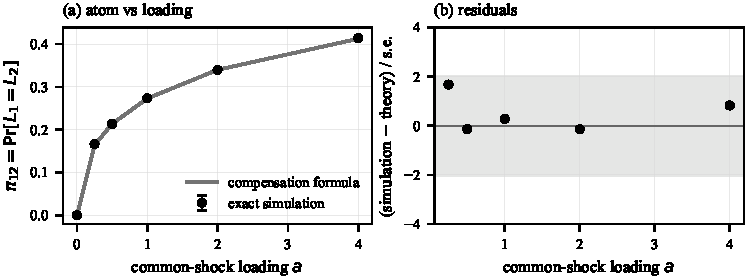
\includegraphics[width=5in]{fig_atom}}
\vspace*{6pt}
\caption{Left: the simultaneous-staleness atom against the common-shock loading,
exact simulation (markers, two standard errors) versus the compensation formula
\eqref{eq:atomformula} evaluated with the closed-form potential density
(line). Right: residuals in units of the simulation standard error; the shaded
band is $\pm2$.}
\label{fig:atom}
\alttext{Left panel: atom probability rising with loading, simulated points
lying on the theoretical curve. Right panel: residuals scattered within two
standard errors of zero.}
\end{figure}

\subsection{The bivariate potential density}

\begin{proposition}\label{prop:homog}
Under Assumption~\ref{ass:equal} the measure $U_{jh}$ is absolutely continuous
off the diagonal, with density satisfying
\begin{equation}
u(c s_j, c s_h) = c^{\alpha-2}\, u(s_j,s_h), \qquad c>0 .
\label{eq:homog}
\end{equation}
\end{proposition}

\begin{theorem}\label{thm:potential}
Let $\alpha=1/2$, $a_j=a_h=a>0$, with $X_j,X_h,Z$ standard $\tfrac12$-stable.
Writing $x_j=s_j-az$ and $x_h=s_h-az$, for $s_j,s_h>0$
\begin{equation}
u(s_j,s_h)
= \pi^{-3/2}\int_{0}^{(s_j\wedge s_h)/a}
\frac{\sqrt{z\,x_j\,x_h}}
     {\big(x_j x_h + z\,(x_j+x_h)\big)^{2}}\; dz .
\label{eq:potential}
\end{equation}
\end{theorem}

The derivation (\ref{app:proofs}) uses the explicit $\tfrac12$-stable
density and evaluates the operational-time integral in closed form. Three checks
are worth recording. Expression \eqref{eq:potential} is homogeneous of degree
$-3/2=\alpha-2$ as Proposition~\ref{prop:homog} requires, verified numerically
to a relative \potHomogMaxErr{} -- machine precision, as befits an identity.
Substituting it into \eqref{eq:atomformula} yields a $t$-free $\pi_{jh}$, as
Proposition~\ref{prop:atom} requires. And it reproduces the simulated atom
(Table~\ref{tab:atom}).

\begin{corollary}\label{cor:log}
As $s_h\to s_j$ the density \eqref{eq:potential} diverges logarithmically:
$u(s,s+\delta) = -\,\pi^{-3/2}c(s)\log\delta + O(1)$ as $\delta\downarrow0$,
with $c(s)>0$.
\end{corollary}

Over \logSingNDecades{} decades, $u(1,1+\delta)$ rises from \logSingFirst{} to
\logSingLast{} in increments of $\logSingIncrMean \pm \logSingIncrSd$ per
decade: a constant increment per decade is the signature of a logarithmic
divergence (Figure~\ref{fig:potential}, left).

\subsection{Resolving the diagonal}

Comparing \eqref{eq:potential} with the exact occupation measure cell by cell
over \potNCells{} cells, agreement away from the diagonal is good: the ratio of
closed form to simulation has median \potOffMedian{} with a 5--95\% range of
\potOffPlo{}--\potOffPhi{} and a mean absolute deviation of \potOffMAD{}\%.

On the diagonal, plain tensor quadrature of the cell fails badly, giving ratios
between \potDiagBoxLo{} and \potDiagBoxHi{} (median \potDiagBoxMedian{}). The
cause is Corollary~\ref{cor:log}: the logarithmic ridge runs through the cell
interior, and symmetric Gauss--Legendre nodes cannot resolve it. Cutting each
diagonal cell along $s_j=s_h$ and integrating the two triangles separately, with
a substitution that annihilates the logarithm at the ridge, moves the ratios to
\potDiagSplitLo{}--\potDiagSplitHi{} (median \potDiagSplitMedian{}); see
Figure~\ref{fig:potential}, right.

This settles a question left open in earlier work on this model, where a
diagonal discrepancy of the same kind had been observed and it was not known
whether it indicated a quadrature failure or an error in the derivation. It is a
quadrature failure.

\begin{figure}[t]
\centerline{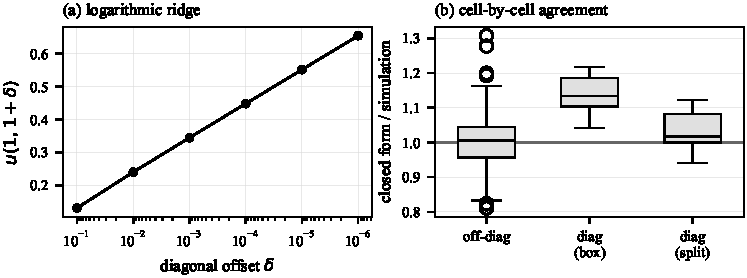
\includegraphics[width=5in]{fig_potential}}
\vspace*{6pt}
\caption{Left: the logarithmic ridge of the bivariate potential density at
$\alpha=1/2$; a constant increment per decade in $\delta$ indicates a
logarithmic divergence. Right: ratio of the closed form \eqref{eq:potential} to
the exact occupation measure, cell by cell. Off the diagonal the two agree.
On the diagonal, plain tensor quadrature fails; splitting the cell along the
ridge repairs it.}
\label{fig:potential}
\alttext{Left panel: values rising linearly as the diagonal offset falls by
decades. Right panel: three box plots, the first and third centred on one and
the middle one biased low.}
\end{figure}

%%%%%%%%%%%%%%%%%%%%%%%%%%%%%%%%%%%%%%%%%%%%%%%%%%%%%%%%%%%%%%%%%%%%%%%%%%%%
\section{Evolution Equations}\label{sec:evol}
%%%%%%%%%%%%%%%%%%%%%%%%%%%%%%%%%%%%%%%%%%%%%%%%%%%%%%%%%%%%%%%%%%%%%%%%%%%%

Write $q(t,\cdot)$ for the density of $(\tilde Y_1(t),\dots,\tilde Y_k(t))$.

\begin{proposition}\label{prop:mixture}
Under Assumption~\ref{ass:equal}, for every $t>0$,
\begin{equation}
q(t,y_1,\dots,y_k)
= \int_{[0,1]^k} \prod_{j=1}^{k} p_j(t s_j, y_j)\ \mu_\alpha(ds),
\label{eq:mixture}
\end{equation}
with $\mu_\alpha$ the $t$-free law of Proposition~\ref{prop:selfsim}.
\end{proposition}

The factors are independent only \emph{conditionally} on the clocks; the
unconditional law is not a product, because $\mu_\alpha$ is not a product
measure when the loadings are positive.

\begin{remark}\label{rem:singular}
It is tempting to differentiate through the time change, writing
$\partial_t p_j(H_j(t),y_j) = \dot H_j(t) G_j p_j$. This is wrong: the range of
$S_j$ is Lebesgue-null, so $\dot H_j=0$ almost everywhere and the right-hand
side vanishes. It is exactly this singularity that forces the nonlocal
formulation of \citet{asc24} and \citet{toa15}. Theorem~\ref{thm:local} obtains
a local equation nonetheless -- not by differentiating the time change, but by
exploiting the exact scaling in \eqref{eq:mixture}.
\end{remark}

\subsection{An exact local equation}

For a probability measure $\mu$ on $[0,1]^k$ with $\int s_j\mu(ds)=m_j$, write
$\mu^{(j)}(ds) := s_j\,\mu(ds)/m_j$ for its \emph{size-biased} version in
coordinate $j$, and let $q^{(j)}$ be obtained by substituting
$\mu_\alpha^{(j)}$ for $\mu_\alpha$ in \eqref{eq:mixture}.

\begin{theorem}\label{thm:local}
Under Assumption~\ref{ass:equal}, $m_j=\alpha$ for every $j$ and
\begin{equation}
\partial_t\, q(t,\cdot) \;=\; \sum_{j=1}^{k}\alpha\; G_j\, q^{(j)}(t,\cdot),
\qquad t>0 ,
\label{eq:local}
\end{equation}
with $G_j$ acting on the $j$th coordinate.
\end{theorem}

The size-biasing constant is the coordinate mean of $\mu_\alpha$, which
Proposition~\ref{prop:beta} fixes at exactly $\alpha$; simulation gives
$\sizeBiasMean$, within \sizeBiasZ{} standard errors. Testing \eqref{eq:local}
against the test function $\varphi(y)=y_1y_2$ turns both sides into the joint
Laplace transform of the clock vector (\ref{app:numerics}); the ratio
of right- to left-hand side lies in $[\localRatioLo, \localRatioHi]$ across five
parameter sets, with a largest discrepancy of \localMaxZ{} standard errors
(Table~\ref{tab:evolution}).

\begin{proposition}\label{prop:kummer}
For $k=1$ with the Ornstein--Uhlenbeck factor \eqref{eq:ou}, equation
\eqref{eq:local} evaluated on the first moment is exactly the derivative
identity
\begin{equation}
\frac{d}{dz}\,\Fone(a;b;z) = \frac{a}{b}\,\Fone(a+1;b+1;z)
\label{eq:kummerid}
\end{equation}
at $(a,b)=(\alpha,1)$, $z=-\kappa t$.
\end{proposition}

\begin{proof}
By \eqref{eq:oumean} the left-hand side of \eqref{eq:local} is
$\partial_t \Fone(\alpha;1;-\kappa t)$. Size-biasing $\Bet(\alpha,1-\alpha)$
gives $\Bet(\alpha+1,1-\alpha)$, whose transform is $\Fone(\alpha+1;2;\cdot)$,
with normalizing constant $B(\alpha+1,1-\alpha)/B(\alpha,1-\alpha)=\alpha$.
Since $Gy=-\kappa y$, the right-hand side is
$-\kappa\alpha\Fone(\alpha+1;2;-\kappa t)$, and \eqref{eq:local} becomes
\eqref{eq:kummerid}.
\end{proof}

We state this to settle what is and is not new. Identity~\eqref{eq:kummerid} is
textbook \citep[Eq.~13.3.15]{nist10}, so Theorem~\ref{thm:local} carries no new
information when $k=1$. Nor does it when $k>1$ with \emph{independent} clocks:
then $\mu_\alpha$ is a product, $\mu_\alpha^{(j)}$ tilts only coordinate $j$,
and \eqref{eq:local} decomposes into $k$ separate copies of
Proposition~\ref{prop:kummer}. The theorem has content precisely when $k>1$ and
the clocks are dependent, because size-biasing one coordinate of a non-product
$\mu_\alpha$ perturbs all $k$ marginals of the tilted measure at once.

\subsection{Failure of tensorization}

\begin{proposition}\label{prop:notensor}
Under Assumption~\ref{ass:equal} with $k\ge2$ and $a_j>0$, the mixing measure
$\mu_\alpha$ is not a product measure. Consequently the evolution equation
obtained by replacing $\mu_\alpha$ with the product of its marginals -- the
tensorization of the one-clock equation -- is incorrect.
\end{proposition}

Non-product-ness follows from Proposition~\ref{prop:atom}: a product measure
with continuous marginals gives the diagonal zero mass, and $\mu_\alpha$ does
not. The quantitative content is in the last column of
Table~\ref{tab:evolution}. Because the marginals are exactly
$\Bet(\alpha,1-\alpha)$, the tensorized prediction is entirely classical,
\begin{equation}
-\sum_j \kappa_j\, \alpha\, \Fone(\alpha+1;2;-\kappa_j t)
\prod_{i\ne j} \Fone(\alpha;1;-\kappa_i t),
\label{eq:tensor}
\end{equation}
and it overstates the true derivative by between
$\tensorRatioLo$ and $\tensorRatioHi$. The common shock is therefore not a
correction one can absorb into marginal calibration, even though
Proposition~\ref{prop:beta} says the marginals themselves are untouched by it.

\begin{table}[t]
\tbl{The local evolution equation \eqref{eq:local} and its tensorization
\eqref{eq:tensor}, at $\alpha=1/2$, $a_1=a_2=1$, $t=1$. $M'(t)$ is estimated by
a central difference on common random paths; ``size-biased'' is the right-hand
side of \eqref{eq:local}.}
{\begin{tabular}{@{}ccrrcrc@{}}
\toprule
$\kappa_1$ & $\kappa_2$ & $M'(t)$ & size-biased & ratio & tensorized & ratio \\
\colrule
1 & 1 & -0.29467 & -0.29188 & 0.9905 & -0.31517 & 1.070 \\
0.5 & 2 & -0.26618 & -0.26684 & 1.0025 & -0.28464 & 1.069 \\
2 & 2 & -0.21689 & -0.21718 & 1.0013 & -0.24019 & 1.107 \\
0.3 & 3 & -0.22355 & -0.22563 & 1.0093 & -0.23680 & 1.059 \\
1 & 0.25 & -0.27931 & -0.27270 & 0.9763 & -0.28342 & 1.015 \\
\botrule
\end{tabular}}
\label{tab:evolution}
\end{table}

%%%%%%%%%%%%%%%%%%%%%%%%%%%%%%%%%%%%%%%%%%%%%%%%%%%%%%%%%%%%%%%%%%%%%%%%%%%%
\section{The Correlation Term Structure Carries No Information}\label{sec:corr}
%%%%%%%%%%%%%%%%%%%%%%%%%%%%%%%%%%%%%%%%%%%%%%%%%%%%%%%%%%%%%%%%%%%%%%%%%%%%

Specialize to the two-component form standard in the staleness literature: an
idiosyncratic and a common component, each on its own clock,
\begin{equation}
P_i(t) = \sigma_i\, Y_i\big(H_i(t)\big) \;+\; a_i\, Y_0\big(H_0(t)\big),
\label{eq:twofactor}
\end{equation}
with $H_i$ the undershoot of a standard $\alpha_i$-stable subordinator, $H_0$
that of a standard $\alpha_c$-stable subordinator, and $Y_0,Y_1,\dots$
independent factors \eqref{eq:ou} with $\sigma_0=1$. Write $\rho_{ih}(\Delta)$
for the correlation of the calendar-time returns over $[t,t+\Delta]$.

\subsection{Under staleness alone the term structure is exactly flat}

\begin{proposition}\label{prop:rhoflat}
Let the factors be driftless Brownian motions, $\kappa_j=0$. Then for every
$t>0$ and every $\Delta>0$,
\begin{equation}
\rho_{ih}(\Delta) \;=\;
\frac{a_i a_h\, \alpha_c}
     {\sqrt{\big(\sigma_i^2\alpha_i + a_i^2\alpha_c\big)
            \big(\sigma_h^2\alpha_h + a_h^2\alpha_c\big)}}\, ,
\label{eq:rhoflat}
\end{equation}
exactly. In particular $\rho_{ih}$ does not depend on the return horizon.
\end{proposition}

The proof is two lines and rests on one exact fact: $\E[H(t)]=\alpha t$, because
$H(t)/t\sim\Bet(\alpha,1-\alpha)$ has mean $\alpha$. Conditionally on the
clocks the Brownian increments have variance $\sigma_i^2\Delta H_i +
a_i^2\Delta H_0$ and covariance $a_ia_h\Delta H_0$; taking expectations
replaces each $\Delta H_j$ by $\alpha_j\Delta$, and $\Delta$ cancels.
Table~\ref{tab:rho} confirms this end to end on simulated prices: across
\rhoNCases{} parameter sets and a \rhoDeltaRatio{}-fold range of horizons the
largest discrepancy is \rhoBrownMaxZ{} standard errors, and the largest spread
of $\rho$ across horizons is \rhoBrownSpread{}.

The economic reading is that \emph{staleness by itself generates no correlation
term structure at all}. Whatever term structure a calibrated model displays
comes from the factor dynamics, not from the staleness mechanism.

\begin{table}[t]
\tbl{Proposition~\ref{prop:rhoflat} tested end to end on simulated prices with
Brownian factors, $\alpha=1/2$.}
{\begin{tabular}{@{}crrrr@{}}
\toprule
Case & $\Delta$ & simulated $\rho$ & s.e. & Eq.~(\ref{eq:rhoflat}) \\
\colrule
1 & 0.02 & 0.51876 & 0.01709 & 0.50000 \\
1 & 0.1 & 0.50334 & 0.00917 & 0.50000 \\
1 & 0.5 & 0.49764 & 0.00549 & 0.50000 \\
1 & 2 & 0.49747 & 0.00435 & 0.50000 \\
2 & 0.02 & 0.22953 & 0.01128 & 0.21693 \\
2 & 0.1 & 0.21426 & 0.00645 & 0.21693 \\
2 & 0.5 & 0.22012 & 0.00527 & 0.21693 \\
2 & 2 & 0.21777 & 0.00491 & 0.21693 \\
3 & 0.02 & 0.41615 & 0.01555 & 0.40000 \\
3 & 0.1 & 0.40250 & 0.00841 & 0.40000 \\
3 & 0.5 & 0.40437 & 0.00525 & 0.40000 \\
3 & 2 & 0.39480 & 0.00521 & 0.40000 \\
\botrule
\end{tabular}}
\label{tab:rho}
\end{table}

\subsection{With mean reversion, the closed form has a domain}

For Ornstein--Uhlenbeck factors, $\mathrm{Var}(Y(u)-Y(v)) =
(\sigma^2/\kappa)(1-e^{-\kappa|u-v|})$, so \eqref{eq:rhoflat} holds with
$\alpha_j\Delta$ replaced by $\kappa_j^{-1}\E[1-e^{-\kappa_j\Delta H_j}]$.

It is worth being explicit about a trap here. One might expect the linearization
$\E[1-e^{-\kappa\Delta H}] \approx \kappa\,\E[\Delta H]=\kappa\alpha\Delta$ to
become exact as $\Delta\downarrow0$, which would make \eqref{eq:rhoflat} the
universal short-horizon limit. It does not. The undershoot increment
$\Delta H$ is zero on most paths and of order $t$ on the rest -- when a trade
finally arrives after a long stale period, the clock jumps by the whole
staleness -- so the relevant scale is $\kappa t$, not $\kappa\Delta$, and the
approximation error does not vanish with $\Delta$. Table~\ref{tab:oulin} shows
the ratio: for $\kappa t \le \rhoKtSmall$ it stays above \rhoLinSmallKt{}, so
\eqref{eq:rhoflat} is accurate; for $\kappa t \ge \rhoKtLarge$ it never exceeds
\rhoLinLargeKt{}, and \eqref{eq:rhoflat} is not usable.

\begin{table}[b]
\tbl{$\E[1-e^{-\kappa\Delta H}] / (\kappa\,\E[\Delta H])$ at $\alpha=1/2$,
$t=1$. A value of one means \eqref{eq:rhoflat} applies. The ratio is governed by
$\kappa t$ and does not approach one as $\Delta\downarrow0$.}
{\begin{tabular}{@{}crrrr@{}}
\toprule
$\kappa t$ & $\Delta=0.02$ & $\Delta=0.1$ & $\Delta=0.5$ & $\Delta=2$ \\
\colrule
0.03 & 0.992 & 0.991 & 0.987 & 0.971 \\
0.1 & 0.974 & 0.972 & 0.958 & 0.907 \\
0.3 & 0.927 & 0.920 & 0.882 & 0.756 \\
1 & 0.791 & 0.775 & 0.680 & 0.450 \\
3 & 0.568 & 0.536 & 0.392 & 0.188 \\
10 & 0.320 & 0.272 & 0.147 & 0.060 \\
30 & 0.171 & 0.117 & 0.051 & 0.020 \\
100 & 0.073 & 0.038 & 0.016 & 0.006 \\
\botrule
\end{tabular}}
\label{tab:oulin}
\end{table}

\subsection{The shape of the term structure is not identified}

An earlier conjecture in this project was that common-shock staleness
\emph{predicts} the shape of $\Delta\mapsto\rho_{ih}(\Delta)$ -- specifically
that it forces the correlation to rise. It does not.

We evaluated \eqref{eq:twofactor} exactly on \sweepN{} parameter combinations
spanning the admissible ranges of
$(\alpha_i,\alpha_h,\alpha_c,\sigma_i,\sigma_h,a_i,a_h,\kappa_i,\kappa_h,\kappa_0)$
over \sweepNdeltas{} horizons from \sweepDeltaLo{} to \sweepDeltaHi{}, and
classified each term structure by its monotonicity. Table~\ref{tab:sweep} and
Figure~\ref{fig:correlation} report the outcome: every class occurs with
substantial frequency and none dominates. The correlation term structure is
free, and no empirical term-structure pattern can confirm or refute
common-shock staleness on its own.

A weaker claim also fails. We had conjectured that the sign of the initial slope
is set by comparing the calendar-time mean-reversion rates $\alpha_j\kappa_j$
and $\alpha_c\kappa_0$. Across the same sweep that rule classifies
\slopeRuleAcc{}\% of cells correctly, which is chance. We record it as refuted.

\begin{table}[t]
\tbl{Shape of $\Delta\mapsto\rho_{ih}(\Delta)$ across \sweepN{} admissible
parameter combinations of model \eqref{eq:twofactor}.}
{\begin{tabular}{@{}lr@{}}
\toprule
Term-structure shape & Share of cells (\%) \\
\colrule
Rising & 21.1 \\
Falling & 22.6 \\
Hump & 31.4 \\
Dip & 24.2 \\
Flat & 0.7 \\
\botrule
\end{tabular}}
\begin{tabnote}
Grid ranges and the classification rule are in \ref{app:numerics}.
\end{tabnote}
\label{tab:sweep}
\end{table}

\begin{figure}[t]
\centerline{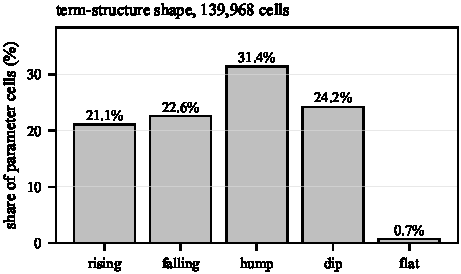
\includegraphics[width=3.1in]{fig_correlation}}
\vspace*{6pt}
\caption{Monotonicity class of the correlation term structure across
\sweepN{} parameter combinations. All four classes occur with comparable
frequency, so the shape carries no identifying information about the staleness
mechanism.}
\label{fig:correlation}
\alttext{Bar chart with four bars of comparable height labelled rising,
falling, hump and dip, plus a negligible flat category.}
\end{figure}

%%%%%%%%%%%%%%%%%%%%%%%%%%%%%%%%%%%%%%%%%%%%%%%%%%%%%%%%%%%%%%%%%%%%%%%%%%%%
\section{Testing the Load-Bearing Assumption}\label{sec:empirics}
%%%%%%%%%%%%%%%%%%%%%%%%%%%%%%%%%%%%%%%%%%%%%%%%%%%%%%%%%%%%%%%%%%%%%%%%%%%%

\subsection{Why $\alpha<1$ is load-bearing}

Every exact statement in Sections~\ref{sec:joint}--\ref{sec:corr} uses
$\alpha\in(0,1)$, and not incidentally. If the inter-trade duration distribution
has a finite mean, then $H(t)/t\to1$ almost surely by the elementary renewal
theorem, the mixing measure $\mu_\alpha$ degenerates to a point mass at
$(1,\dots,1)$, the Beta law \eqref{eq:beta} disappears, \eqref{eq:mixture}
collapses to $q(t,\cdot)=\prod_j p_j(t,\cdot)$, and the process is Markov again.
Staleness does not vanish -- prices are still frozen between trades -- but it
stops being a non-negligible fraction of any horizon, and the non-Markovian
apparatus becomes an asymptotically empty elaboration.

Concretely the model requires $\PP[\tau>x]\sim Cx^{-\alpha}$ with $\alpha<1$ for
the inter-trade duration $\tau$: an infinite mean waiting time. This is the
assumption the call for papers cites as the empirical motivation for the
program. It is testable and the tests are cheap.

\subsection{Data}

\begin{itemlist}
\item \textbf{Cryptocurrency.} Binance spot aggregated-trade records for
\cryptoNsym{} USDT pairs over one full UTC day, spanning \cryptoVolDecades{}
orders of magnitude in 24-hour turnover (from \cryptoVolLo{} to \cryptoVolHi{}
USDT): \cryptoTotalOrders{} orders built from \cryptoTotalFills{} individual
fills, timestamped to the millisecond. Each record carries the first and last
raw trade identifiers, so the number of fills behind every order is known
exactly and both event definitions are available from one download.

\item \textbf{Vietnamese equities.} Trade-by-trade records from the Ho Chi Minh
Stock Exchange for \hoseNsym{} symbols over one continuous morning session,
\hoseTotalTicks{} prints in total, with median inter-trade gaps ranging from
\hoseGapLo{} to \hoseGapHi{} seconds. HOSE timestamps have one-second
resolution, and between \hoseTieLo{}\% and \hoseTieHi{}\% of consecutive prints
tie.
\end{itemlist}

The two markets are deliberately opposite: a continuously traded
twenty-four-hour venue with millisecond stamps, and a session-based equity
market with second stamps. Estimation procedures -- the Hill estimator
\citep{hil75} with a Hill-plot plateau rule, an assumption-free running-mean
diagnostic, burst aggregation, diurnal adjustment, and the
Clauset--Shalizi--Newman goodness-of-fit test \citep{cla09} -- are in
\ref{app:numerics}.

\subsection{The tail index is a property of the event definition}

A marketable order executed against several resting orders generates several
prints at one timestamp. Counting each fill as an event injects zero durations,
which enlarges the sample and pushes the Hill threshold deep into the body of
the distribution. Table~\ref{tab:eventdef} recomputes the tail index under
successively coarser event definitions on the identical data.

\begin{table}[t]
\tbl{Duration tail index by event definition, Binance spot, \cryptoNsym{}
pairs. Every column uses the same underlying trade records.}
{\begin{tabular}{@{}lrrr@{}}
\toprule
Event definition & median $\hat\alpha$ & share $\hat\alpha<1$ (\%) & pairs \\
\colrule
individual fills & 0.24 & 76 & 21 \\
orders (aggregated fills) & 1.19 & 38 & 21 \\
orders merged within $0.1$\,s & 1.51 & 10 & 21 \\
orders merged within $1$\,s & 1.61 & 5 & 21 \\
orders merged within $5$\,s & 2.42 & 5 & 21 \\
orders, diurnally adjusted & 1.28 & 35 & 20 \\
\botrule
\end{tabular}}
\label{tab:eventdef}
\end{table}

The median index rises monotonically from \cryptoAlphaFillMed{} at fill level to
\cryptoAlphaOrderMed{} at order level and \cryptoAlphaWbMed{} after merging
within one second, and the share of pairs with $\hat\alpha<1$ falls from
\cryptoAlphaFillFrac{}\% to \cryptoAlphaOrderFrac{}\% to
\cryptoAlphaWbFrac{}\%. Figure~\ref{fig:eventdef} shows the whole distribution.

This is diagnostic, not merely inconvenient. A tail index is an asymptotic
property of the duration distribution and is invariant under coarsening of the
event definition; a statistic that moves monotonically and without bound as the
definition is coarsened is measuring the microstructure of order execution, not
the tail of a trading-time distribution. The apparent infinite-mean waiting
times in the raw data are an artifact of the finest event definition, and they
are largest where markets are most active: fills per order range from
\cryptoFillRatioLo{} to \cryptoFillRatioHi{} across the sample, and it is the
liquid pairs that burst.

\begin{figure}[t]
\centerline{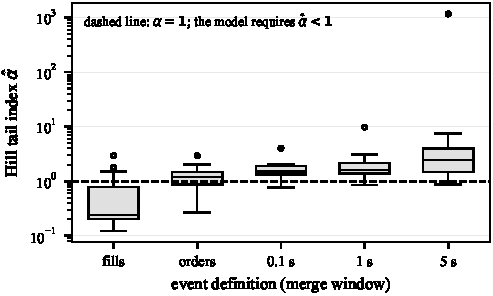
\includegraphics[width=3.3in]{fig_event_definition}}
\vspace*{6pt}
\caption{Distribution across \cryptoNsym{} Binance pairs of the Hill tail index
under successively coarser event definitions, from individual fills through
orders to orders merged within a window. The model requires the index to lie
below the dashed line. A genuine tail index would be invariant to this choice.}
\label{fig:eventdef}
\alttext{Box plots on a logarithmic axis showing the tail index rising steadily
from well below one at fill level to well above one at coarser event
definitions.}
\end{figure}

\subsection{The diurnal cycle does the rest}

A Poisson process whose rate varies over the day produces durations that are a
\emph{mixture} of exponentials, and mixtures of exponentials have
heavier-than-exponential tails. Any index estimated on a full trading day
therefore confounds tail behavior with the activity cycle. The cycle is large:
the smoothed intraday profile of mean duration varies by a median factor of
\cryptoDiurnalMed{} across pairs, and by up to \cryptoDiurnalHi{}.

Dividing durations by that profile changes two things. The assumption-free
running-mean ratio -- which drifts upward without bound when the mean is
infinite -- tightens from a raw range of
\cryptoRMrawLo{}--\cryptoRMrawHi{} to \cryptoRMadjLo{}--\cryptoRMadjHi{}, so
the apparent non-convergence was the activity cycle rather than an infinite
mean. And the median tail index rises to \cryptoAlphaDeseasMed{}, with
\cryptoAlphaDeseasFrac{}\% of pairs below one. Figure~\ref{fig:deseason} traces
each symbol individually through the adjustment.

\begin{figure}[t]
\centerline{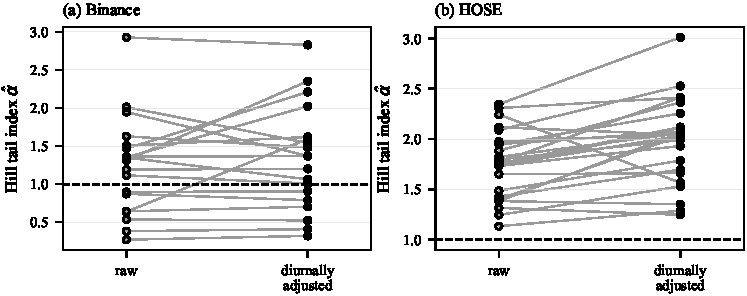
\includegraphics[width=5in]{fig_deseason}}
\vspace*{6pt}
\caption{Effect of removing the diurnal activity cycle on the estimated tail
index, symbol by symbol, in both markets. The dashed line is $\alpha=1$, below
which the model requires every point to lie.}
\label{fig:deseason}
\alttext{Two panels of paired points connected by lines, with most values
rising above the dashed line at one after diurnal adjustment.}
\end{figure}

\subsection{The decisive test: is anything both a power law and infinite-mean?}

The Hill estimator returns a number whether or not the tail is a power law, and
it uses a threshold chosen by rule rather than fitted. The
Clauset--Shalizi--Newman procedure removes both objections: it fits the
threshold $x_{\min}$ and the index by maximum likelihood and calibrates the
Kolmogorov--Smirnov distance against parametric bootstrap replications, so a
small $p$-value rejects the power-law hypothesis itself.

Applying it to every series in both markets gives the paper's sharpest result.
Among the \cryptoOrderTested{} cryptocurrency pairs, the number that are both a
plausible power law ($p\ge0.10$) and infinite-mean ($\hat\alpha<1$) is
\cryptoOrderSurvivors{}; after diurnal adjustment it is
\cryptoDeseasSurvivors{}. Among the \hoseTested{} HOSE symbols it is
\hoseSurvivors{}. The fitted indices are not marginal: their median is
\cryptoOrderCsnMedian{} at order level and \cryptoDeseasCsnMedian{} after
adjustment, with a minimum across all adjusted series of \cryptoDeseasCsnMin{}.

Two points of interpretation. First, the fitted threshold $x_{\min}$ always
falls above the zero durations, so the positive-duration sample is the same
under the fill- and order-level definitions and the test is properly a statement
about the order-level series; the fill-level zeros sit in the body below
$x_{\min}$ by construction. That is precisely why the Hill estimator and this
procedure disagree so sharply: Hill's threshold is a fixed fraction of $n$ and
the zeros inflate $n$, whereas a fitted $x_{\min}$ is immune to them. Second,
some series do have a fitted index below one -- the smallest at order level is
\cryptoOrderCsnMin{} -- but in every such case the power-law hypothesis is
itself rejected, so the index estimates the tail exponent of a distribution that
has none.

The pairs that appeared to support $\alpha<1$ under the Hill estimator are
precisely those for which a properly fitted threshold puts the index above one,
or for which the power law is rejected outright. Per-symbol detail is in
Tables~\ref{tab:crypto} and \ref{tab:hose}.

\subsection{Cross-section: illiquid names do not have heavier tails}

If staleness were a tail phenomenon, illiquid names would have \emph{smaller}
indices: their durations would be not merely longer but heavier-tailed. The
model's cross-sectional prediction is a strong negative correlation between
typical gap length and $\hat\alpha$. We find the opposite sign in both markets.

On Binance the correlation between the log median gap and the tail index is
\cryptoCorrOrder{} ($p=\cryptoCorrPOrder$) at order level and
\cryptoCorrDeseas{} ($p=\cryptoCorrPDeseas$) after diurnal adjustment. On HOSE
it is \hoseSecondCorr{} ($p=\hoseSecondCorrP$, $n=\hoseSecondN$) and
\hoseDeseasCorr{} ($p=\hoseDeseasCorrP$) respectively. Figure~\ref{fig:cross}
shows both cross-sections. Illiquid names have longer typical gaps and the
same, or slightly lighter, tails. Staleness in these markets is a scale effect,
not a tail effect.

\begin{figure}[t]
\centerline{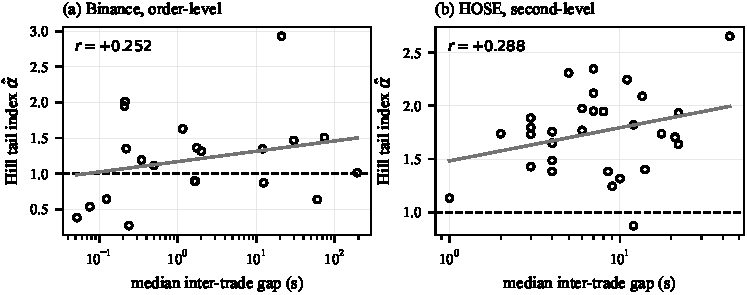
\includegraphics[width=5in]{fig_cross_section}}
\vspace*{6pt}
\caption{Tail index against median inter-trade gap. The model requires all
points below the dashed line and a steeply negative slope; the fitted slope is
positive in both markets.}
\label{fig:cross}
\alttext{Two scatter plots of tail index against median gap on logarithmic
axes, with mildly upward-sloping fitted lines and nearly all points above the
dashed reference at one.}
\end{figure}

\begin{table}[p]
\tbl{Binance spot, one UTC day. ``fill'', ``order'' and ``adj.'' are Hill
indices at fill level, order level and after diurnal adjustment; CSN $p$ is the
Clauset--Shalizi--Newman goodness-of-fit $p$-value for the order-level series.}
{\small\begin{tabular}{@{}lrrrrrrrr@{}}
\toprule
Pair & 24h volume & orders & median & fills & \multicolumn{3}{c}{Hill $\hat\alpha$} & CSN \\
 & (USDT) & & gap (s) & /order & fill & order & adj. & $p$ \\
\colrule
BTC & 469{,}369{,}949 & 185{,}781 & 0.346 & 2.91 & 0.24 & 1.19 & 1.20 & 0.00 \\
ETH & 200{,}616{,}691 & 107{,}772 & 0.496 & 3.80 & 0.20 & 1.12 & 1.01 & 0.00 \\
XPL & 177{,}849{,}163 & 237{,}525 & 0.213 & 2.23 & 1.78 & 2.01 & 1.54 & 0.47 \\
ALLO & 103{,}539{,}172 & 175{,}614 & 0.221 & 3.21 & 0.24 & 1.35 & 2.02 & 0.41 \\
PLUME & 79{,}828{,}878 & 170{,}520 & 0.210 & 2.02 & 0.77 & 1.95 & 1.37 & 0.07 \\
SOL & 62{,}565{,}619 & 48{,}469 & 1.159 & 2.88 & 0.17 & 1.63 & 1.48 & 0.00 \\
XRP & 35{,}249{,}120 & 29{,}505 & 1.757 & 3.08 & 0.17 & 1.36 & 1.37 & 0.00 \\
HEMI & 23{,}990{,}471 & 118{,}193 & 0.124 & 3.79 & 0.23 & 0.64 & 0.70 & 0.70 \\
LINK & 12{,}732{,}843 & 120{,}988 & 0.076 & 3.25 & 0.23 & 0.53 & 0.52 & 0.00 \\
BICO & 8{,}441{,}674 & 94{,}197 & 0.052 & 1.98 & 0.23 & 0.38 & 0.41 & 0.00 \\
SPCXB & 4{,}934{,}827 & 18{,}139 & 1.674 & 1.83 & 0.69 & 0.89 & 0.91 & 0.00 \\
TRUMP & 3{,}008{,}634 & 7{,}032 & 1.630 & 2.74 & 0.16 & 0.90 & 0.91 & 0.00 \\
SYRUP & 1{,}754{,}859 & 6{,}168 & 2.001 & 2.64 & 0.15 & 1.31 & 2.35 & 0.00 \\
RSR & 235{,}711 & 1{,}944 & 30.000 & 1.31 & 1.48 & 1.47 & 2.21 & 0.00 \\
AMP & 142{,}844 & 2{,}135 & 12.015 & 1.30 & 0.71 & 1.35 & 1.06 & 0.09 \\
A & 85{,}770 & 2{,}449 & 0.238 & 1.69 & 0.27 & 0.27 & 0.32 & 0.00 \\
LQTY & 51{,}617 & 1{,}212 & 12.440 & 1.77 & 0.12 & 0.87 & 0.79 & 0.81 \\
XVS & 30{,}203 & 3{,}575 & 21.009 & 1.20 & 2.93 & 2.93 & 2.83 & 0.00 \\
PYPLB & 18{,}279 & 627 & 73.871 & 1.11 & 1.51 & 1.51 & 1.62 & 0.09 \\
SMHB & 10{,}982 & 516 & 60.000 & 1.03 & 0.64 & 0.64 & 1.59 & 0.02 \\
GSB & 4{,}098 & 249 & 193.519 & 1.02 & 1.01 & 1.01 & --- & 0.04 \\
\botrule
\end{tabular}}
\label{tab:crypto}
\end{table}

\begin{table}[p]
\tbl{HOSE, one continuous morning session. ``print'' counts every print,
``second'' merges prints sharing a timestamp, ``adj.'' additionally removes the
intraday activity profile.}
{\small\begin{tabular}{@{}lrrrrrrr@{}}
\toprule
Symbol & prints & ties & median & \multicolumn{3}{c}{Hill $\hat\alpha$} & CSN \\
 & & (\%) & gap (s) & print & second & adj. & $p$ \\
\colrule
SHB & 2{,}448 & 12 & 1.0 & 1.12 & 1.13 & 1.29 & 0.00 \\
SSI & 2{,}840 & 20 & 2.0 & 1.45 & 1.74 & 2.11 & 0.06 \\
HPG & 2{,}009 & 12 & 3.0 & 1.44 & 1.73 & 1.93 & 0.00 \\
MSN & 1{,}064 & 9 & 3.0 & 1.28 & 1.43 & 1.70 & 0.00 \\
VIX & 2{,}112 & 12 & 3.0 & 1.55 & 1.80 & 1.99 & 0.00 \\
TCB & 2{,}071 & 9 & 3.0 & 1.92 & 1.89 & 2.36 & 0.00 \\
DXG & 1{,}120 & 12 & 4.0 & 1.40 & 1.38 & 2.06 & 0.05 \\
FPT & 1{,}459 & 9 & 4.0 & 1.91 & 1.49 & 1.79 & 0.00 \\
VNM & 1{,}294 & 11 & 4.0 & 1.66 & 1.65 & 1.66 & 0.00 \\
GEX & 1{,}236 & 10 & 4.0 & 1.75 & 1.76 & 2.12 & 0.00 \\
MBB & 1{,}323 & 8 & 5.0 & 1.90 & 2.31 & 2.41 & 0.03 \\
VCB & 956 & 7 & 6.0 & 1.78 & 1.77 & 2.42 & 0.00 \\
VPB & 978 & 7 & 6.0 & 1.85 & 1.97 & 2.05 & 0.01 \\
VND & 897 & 6 & 7.0 & 2.31 & 2.35 & 3.01 & 0.00 \\
BID & 864 & 10 & 7.0 & 1.85 & 1.95 & 2.07 & 0.00 \\
CTG & 811 & 5 & 7.0 & 2.13 & 2.12 & 2.05 & 0.00 \\
STB & 658 & 12 & 8.0 & 1.95 & 1.95 & 2.26 & 0.00 \\
DIG & 535 & 4 & 8.5 & 1.38 & 1.38 & 1.35 & 0.00 \\
GAS & 450 & 12 & 9.0 & 1.08 & 1.25 & 1.53 & 0.46 \\
KDH & 398 & 5 & 10.0 & 1.32 & 1.32 & 1.25 & 0.20 \\
NLG & 398 & 6 & 11.0 & 2.28 & 2.24 & 1.57 & 0.06 \\
MWG & 512 & 8 & 12.0 & 1.80 & 1.82 & 2.06 & 0.02 \\
SBT & 231 & 2 & 12.0 & 0.88 & 0.88 & --- & 0.91 \\
TCH & 435 & 4 & 13.5 & 2.37 & 2.09 & 2.53 & 0.00 \\
POW & 372 & 5 & 14.0 & 1.40 & 1.40 & 2.03 & 0.62 \\
PVD & 328 & 6 & 17.5 & 1.74 & 1.74 & 2.03 & 0.09 \\
HSG & 225 & 0 & 21.0 & 1.71 & 1.71 & --- & 0.13 \\
HHV & 223 & 5 & 22.0 & 1.30 & 1.64 & --- & 0.00 \\
DCM & 298 & 6 & 22.0 & 1.94 & 1.93 & --- & 0.30 \\
REE & 151 & 2 & 44.0 & 2.65 & 2.65 & --- & --- \\
\botrule
\end{tabular}}
\label{tab:hose}
\end{table}

\subsection{Summary}

\begin{arabiclist}
\item The estimated duration tail index rises monotonically as the event
definition is coarsened, from \cryptoAlphaFillMed{} at fill level to
\cryptoAlphaWcMed{} at a five-second merge. A genuine tail index would not move.
\item Removing the diurnal activity cycle raises it further, to
\cryptoAlphaDeseasMed{}, and removes the apparent non-convergence of running
means.
\item Once the tail threshold is fitted rather than chosen by rule, no series in
either market -- \cryptoOrderTested{} cryptocurrency pairs and \hoseTested{}
equities -- is both a plausible power law and infinite-mean.
\item Cross-sectionally the index rises, not falls, with illiquidity, in both
markets.
\end{arabiclist}

We therefore find no empirical anchor for the inverse-stable-subordinator
staleness mechanism as it is usually motivated.

%%%%%%%%%%%%%%%%%%%%%%%%%%%%%%%%%%%%%%%%%%%%%%%%%%%%%%%%%%%%%%%%%%%%%%%%%%%%
\section{Discussion: Staleness as a Scale Effect}\label{sec:discussion}
%%%%%%%%%%%%%%%%%%%%%%%%%%%%%%%%%%%%%%%%%%%%%%%%%%%%%%%%%%%%%%%%%%%%%%%%%%%%

\subsection{What survives}

The theory splits cleanly along the line the data draw.

\emph{Survives.} Everything that follows from \emph{dependence} rather than from
\emph{scaling}. Proposition~\ref{prop:atom} and Theorem~\ref{thm:atomformula}
use only that the clocks share jumps, and hold for any multivariate subordinator
with a common-shock component whatever the tail index. So does
Proposition~\ref{prop:notensor}: marginal operators never tensorize in the
presence of a common shock, because the diagonal atom is invisible to each
marginal separately. Combined with Proposition~\ref{prop:beta} -- marginals are
blind to the common shock -- this identifies the atom as the object worth
estimating, and it is the part of this paper we expect to be reusable.

\emph{Does not survive.} Everything that uses $\alpha\in(0,1)$: the exact Beta
mixing law, the self-similarity of Proposition~\ref{prop:selfsim}, the mixture
representation \eqref{eq:mixture}, and hence Theorem~\ref{thm:local}, which is
derived from the scaling and not from the time change
(Remark~\ref{rem:singular}). Proposition~\ref{prop:rhoflat} likewise uses
$\E[H(t)]=\alpha t$.

\subsection{The repair the data suggest}

The HOSE cross-section is not merely a rejection; it has a shape. Median gaps
span \hoseGapLo{} to \hoseGapHi{} seconds while indices stay in a band around
\hoseSecondMed{} with no downward trend. Illiquidity moves the \emph{scale} of
the duration distribution and leaves its \emph{tail} alone.

The clock family that reproduces this is the tempered stable subordinator
\citep{ros07}. Replace each $X_j$ by a subordinator with L\'evy measure
\begin{equation}
\Pi_j(dz) = \frac{\alpha}{\Gamma(1-\alpha)}\,z^{-1-\alpha}\,e^{-\theta_j z}\,dz,
\qquad \theta_j>0,
\end{equation}
so that
\begin{equation}
\psi_j(\lambda) = (\lambda+\theta_j)^{\alpha} - \theta_j^{\alpha},
\qquad
\E[X_j(1)] = \psi_j'(0) = \alpha\,\theta_j^{\alpha-1} < \infty .
\label{eq:tempered}
\end{equation}
Three properties match the data point for point.

\begin{arabiclist}
\item \textbf{A common index and an asset-specific scale.} All assets share
$\alpha$; heterogeneity enters only through $\theta_j$, which sets the duration
scale $1/\theta_j$. That is the observed cross-section.
\item \textbf{Finite mean.} By \eqref{eq:tempered} the expected duration is
finite for every $\theta_j>0$, consistent with the running-mean ratios of
Section~\ref{sec:empirics} once the diurnal cycle is removed.
\item \textbf{A crossover, not an exponent.} For $t\ll1/\theta_j$ the tempering
is invisible and $H_j(t)/t$ is approximately $\Bet(\alpha,1-\alpha)$: at
intraday horizons the process behaves exactly like the stable clock analyzed
above. For $t\gg1/\theta_j$, $H_j(t)/t\to1$ and the process is effectively
Markov. Staleness becomes a phenomenon of a specific estimable time scale rather
than a self-similar fraction of every horizon.
\end{arabiclist}

The common-shock construction \eqref{eq:clock} carries over unchanged, so the
simultaneity atom and Theorem~\ref{thm:atomformula} continue to hold with the
tempered L\'evy tail in place of \eqref{eq:levytail}. What is lost is exact
self-similarity, and with it Theorem~\ref{thm:local}: the mixing measure then
depends on $t$, and the local equation survives only in the short-horizon
regime.

\begin{question}\label{q:tempered}
For a multivariate tempered stable clock $S_j=X_j+a_jZ$ with common index
$\alpha$ and asset-specific tempering rates $\theta_j$, what governing equation
does the law of $(Y_1(H_1(t)),\dots,Y_k(H_k(t)))$ satisfy, and does the
crossover at $t\sim1/\theta_j$ admit a uniform description?
\end{question}

\subsection{Implications for the non-Markovian factor program}

Three conclusions for the wider program.

First, the two strands the program seeks to unify may not need the same
mathematics. Long memory in volatility is empirically robust \citep{gat18}.
Infinite-mean inter-trade durations are not: on the evidence here they are an
artifact of fill-level data and the diurnal cycle. A framework coupling the two
through a shared index $\alpha$ imposes a constraint the data do not support.

Second, staleness itself is not in question. Prices do freeze between trades and
excess idle time is a real, measurable feature of equity data \citep{ban17}.
What is in question is the specific mechanism of an $\alpha$-stable trading
clock with $\alpha<1$. Non-exponential durations with finite mean -- Weibull,
log-normal, tempered stable, or the self-exciting arrival models of
\citet{bac13} and \citet{eng98} -- are compatible with everything we observe and
produce staleness without infinite mean.

Third, the multivariate structure is where the mathematical interest remains.
The simultaneity atom is invisible to any single asset's duration distribution
(Proposition~\ref{prop:beta}) and not recoverable from the correlation term
structure (Proposition~\ref{prop:rhoflat} and Table~\ref{tab:sweep}); it can be
identified only from joint staleness patterns. Theorem~\ref{thm:atomformula}
makes it computable. That is a well-posed estimation problem, unaffected by our
negative tail result, and it does not appear to have been attempted.

%%%%%%%%%%%%%%%%%%%%%%%%%%%%%%%%%%%%%%%%%%%%%%%%%%%%%%%%%%%%%%%%%%%%%%%%%%%%
\section{Conclusion}
%%%%%%%%%%%%%%%%%%%%%%%%%%%%%%%%%%%%%%%%%%%%%%%%%%%%%%%%%%%%%%%%%%%%%%%%%%%%

We have built the multivariate inverse-subordination factor model that the
additive-subordination literature identified as its open next step and
characterized it: exact self-similarity of the clock vector, generalized arcsine
marginals that are blind to the common shock, an atom of simultaneous staleness
with a compensation-formula representation, a closed-form bivariate potential
density at $\alpha=1/2$ whose logarithmic diagonal ridge explains a numerical
discrepancy previously left open, an exact local evolution equation driven by
size-biased mixing measures that reduces to a classical confluent hypergeometric
identity for one clock, and a quantified failure of the marginal operators to
tensorize.

We have also reported negative results a reader needs in order to use any of
this. Under staleness alone the correlation term structure is exactly flat, and
once mean reversion is added its shape is unidentified: all four monotonicity
classes occur with comparable frequency across \sweepN{} parameter
combinations, and a slope-sign rule we had conjectured performs at chance. Most
importantly, the mechanism's load-bearing assumption -- a duration tail index
below one -- has no empirical support in either market we tested. The estimated
index is a property of the event definition and the diurnal cycle, and once the
tail threshold is fitted properly no series is both a plausible power law and
infinite-mean.

The constructive reading is that staleness in modern electronic markets is a
scale effect rather than a tail effect, and that a tempered stable clock with a
common index and asset-specific tempering rates is the model the data describe.
The dependence results of this paper transfer to that setting unchanged; the
scaling results do not, and finding the governing equations for the tempered
multivariate case is the problem we would work on next.

\appendix

%%%%%%%%%%%%%%%%%%%%%%%%%%%%%%%%%%%%%%%%%%%%%%%%%%%%%%%%%%%%%%%%%%%%%%%%%%%%
\section{Proofs}\label{app:proofs}
%%%%%%%%%%%%%%%%%%%%%%%%%%%%%%%%%%%%%%%%%%%%%%%%%%%%%%%%%%%%%%%%%%%%%%%%%%%%

\subsection*{Proof of Proposition~\ref{prop:selfsim}}

A standard $\alpha$-stable subordinator satisfies
$(X(c^{\alpha}u))_{u\ge0} \eqd (c\,X(u))_{u\ge0}$. Under
Assumption~\ref{ass:equal} all of $X_1,\dots,X_k,Z$ share the index and are
independent, so the scaling holds jointly for the vector, hence for
$S=(S_1,\dots,S_k)$. Substituting $u=c^{\alpha}v$,
\begin{equation}
L_j(ct) = \inf\{u: S_j(u)>ct\}
        = c^{\alpha}\inf\{v: S_j(c^{\alpha}v)>ct\}
        \eqd c^{\alpha}\inf\{v: c\,S_j(v)>ct\}
        = c^{\alpha}L_j(t),
\end{equation}
jointly in $j$, since one realization of the scaled process serves every
coordinate. Hence $H_j(ct)=S_j(L_j(ct)-)\eqd c\,S_j(L_j(t)-)=c\,H_j(t)$,
jointly. Taking $c=1/t$ gives the last claim. \qed

\subsection*{Proof of Proposition~\ref{prop:kummertransform}}

By Proposition~\ref{prop:beta}, $H(t)=tB$ with $B\sim\Bet(\alpha,1-\alpha)$. The
moment generating function of $\Bet(a,b)$ is $\Fone(a;a+b;\cdot)$
\citep[Sec.~13]{nist10}; with $a=\alpha$, $b=1-\alpha$ we have $a+b=1$, giving
\eqref{eq:kummertransform}. For \eqref{eq:oumean}, condition on $H_j(t)$, which
is independent of $Y_j$, and use $\E[Y(u)|Y(0)=y]=ye^{-\kappa u}$. \qed

\subsection*{Proof of Proposition~\ref{prop:atom} and
Theorem~\ref{thm:atomformula}}

Since $X_j$ and $X_h$ are independent stable subordinators they a.s. share no
jump time, so $S_j$ and $S_h$ jump simultaneously precisely at the jump times of
$Z$. If $L_j(t)=L_h(t)=u$, both coordinates cross $t$ at $u$, forcing
$\Delta Z(u)>0$. Conversely, at a jump time $u$ of $Z$ with pre-jump position
$(s_j,s_h)$ and jump size $\zeta$, both cross $t$ iff $s_j,s_h\le t$ and
\begin{equation}
\zeta > \frac{t-s_j}{a_j} \vee \frac{t-s_h}{a_h}.
\end{equation}
The jump times and sizes of $Z$ form a Poisson point process with intensity
$du\,\Pi_{\alpha_c}(d\zeta)$; the pre-jump position is
$\mathcal{F}_{u-}$-measurable and the jump size independent of it, so the
compensation formula gives
\begin{align}
\PP\big[L_j(t)=L_h(t)\big]
&= \int_0^\infty \E\left[\ind\{S_j(u)\le t,\, S_h(u)\le t\}\;
   \bar\Pi_{\alpha_c}\!\Big(\tfrac{t-S_j(u)}{a_j}\vee
   \tfrac{t-S_h(u)}{a_h}\Big)\right] du \nonumber\\
&= \int_{[0,t]^2}
   \bar\Pi_{\alpha_c}\!\Big(\tfrac{t-s_j}{a_j}\vee\tfrac{t-s_h}{a_h}\Big)\,
   U_{jh}(ds_j,ds_h),
\end{align}
which is \eqref{eq:atomformula}. Positivity holds because
$\bar\Pi_{\alpha_c}>0$ on $(0,\infty)$ by \eqref{eq:levytail} and $U_{jh}$
charges $[0,t]^2$; $\pi_{jh}<1$ because with positive probability $X_j$ alone
carries $S_j$ across $t$ strictly before $S_h$ crosses. Independence of $t$
follows from Proposition~\ref{prop:selfsim}, the event being invariant under the
joint scaling \eqref{eq:selfsim}. If $a_ja_h=0$, at least one coordinate shares
no jump with the other and simultaneous crossing has probability zero. \qed

\subsection*{Proof of Proposition~\ref{prop:homog}}

For Borel $B\subset(0,\infty)^2$ and $c>0$, substituting $v=c^{\alpha}w$ and
using the joint scaling above,
\begin{equation}
U_{jh}(cB) = \int_0^\infty \PP\big[(S_j,S_h)(v)\in cB\big]\,dv
= c^{\alpha}\!\int_0^\infty \PP\big[c\,(S_j,S_h)(w)\in cB\big]\,dw
= c^{\alpha}\,U_{jh}(B).
\end{equation}
Applying this to a small box of measure $|B|$, so $|cB|=c^2|B|$, and letting
$|B|\to0$ gives \eqref{eq:homog} at every Lebesgue point. \qed

\subsection*{Proof of Theorem~\ref{thm:potential}}

The standard $\tfrac12$-stable subordinator, with Laplace exponent
$\lambda^{1/2}$, has density
\begin{equation}
f_u(x) = \frac{u}{2\sqrt{\pi}}\,x^{-3/2}\,e^{-u^{2}/(4x)},
\qquad x>0,
\label{eq:halfstable}
\end{equation}
as follows from $\int_0^\infty e^{-\lambda x}f_u(x)dx = e^{-u\sqrt\lambda}$.
Conditioning on the common component and using independence, the joint density
of $(S_j(u),S_h(u))$ at $(s_j,s_h)$ is
$\int_0^{(s_j\wedge s_h)/a} f_u(x_j)f_u(x_h)f_u(z)\,dz$ with $x_j=s_j-az$,
$x_h=s_h-az$; the substitution $w=az$ for the scaled shock contributes no net
Jacobian, and the upper limit enforces $x_j,x_h>0$. Integrating over operational
time and exchanging the order of integration,
\begin{equation}
u(s_j,s_h) = \int_0^{(s_j\wedge s_h)/a}
\left[\int_0^\infty f_u(x_j)f_u(x_h)f_u(z)\,du\right] dz .
\end{equation}
Inserting \eqref{eq:halfstable} three times, the inner integral is
\begin{equation}
\frac{(z\,x_j\,x_h)^{-3/2}}{8\pi^{3/2}}
\int_0^\infty u^{3} e^{-u^{2}C/4}\,du,
\qquad
C := \frac1z + \frac1{x_j} + \frac1{x_h}.
\end{equation}
Since $\int_0^\infty u^3 e^{-\lambda u^2}du = 1/(2\lambda^2)$, taking
$\lambda=C/4$ gives $8/C^{2}$, so the inner integral equals
$\pi^{-3/2}(z x_j x_h)^{-3/2} C^{-2}$. Writing
$C = (x_jx_h + z(x_j+x_h))/(z x_j x_h)$ turns this into
$\pi^{-3/2}\sqrt{z x_j x_h}\,(x_jx_h+z(x_j+x_h))^{-2}$; integrating in $z$ gives
\eqref{eq:potential}. \qed

\subsection*{Proof of Corollary~\ref{cor:log}}

Set $s_j=s$, $s_h=s+\delta$, and let $\epsilon := x_j = s-az$, so
$x_h=\epsilon+\delta$ and $dz=-d\epsilon/a$. As $\epsilon\downarrow0$ we have
$z\to s/a$, and $x_jx_h = O(\epsilon^2+\epsilon\delta)$ is negligible against
$z(x_j+x_h)\asymp(s/a)(2\epsilon+\delta)$, so the integrand of
\eqref{eq:potential} behaves like
\begin{equation}
\frac{\sqrt{z}\,\sqrt{\epsilon(\epsilon+\delta)}}{z^{2}(2\epsilon+\delta)^{2}}
\;\asymp\;
\frac{a^{3/2}}{s^{3/2}}\,
\frac{\sqrt{\epsilon(\epsilon+\delta)}}{(2\epsilon+\delta)^{2}} .
\end{equation}
For $\epsilon\gg\delta$ this is $\asymp1/(4\epsilon)$, so the range
$\delta\lesssim\epsilon\lesssim s$ contributes
$\asymp\tfrac14 a^{1/2}s^{-3/2}\log(s/\delta)$ to $\int d\epsilon/a$, while
$\epsilon\lesssim\delta$ contributes $O(1)$. Hence
$u(s,s+\delta)=-\pi^{-3/2}c(s)\log\delta+O(1)$ with
$c(s)=\tfrac14a^{1/2}s^{-3/2}>0$. \qed

\subsection*{Proof of Theorem~\ref{thm:local}}

By Proposition~\ref{prop:mixture} and dominated convergence,
\begin{equation}
\partial_t q(t,y)
= \int_{[0,1]^k} \sum_{j=1}^{k} s_j\,
\big(\partial_r p_j\big)(t s_j, y_j)
\prod_{i\ne j} p_i(t s_i, y_i)\ \mu_\alpha(ds).
\end{equation}
Each $Y_j$ is Feller, so $\partial_r p_j = G_j p_j$, and $G_j$ acts only on the
$j$th coordinate, hence commutes with the $s$-integration:
\begin{equation}
\partial_t q(t,y)
= \sum_{j=1}^{k} G_j \int_{[0,1]^k} s_j
\prod_{i=1}^{k} p_i(t s_i, y_i)\ \mu_\alpha(ds).
\end{equation}
By Proposition~\ref{prop:beta} the $j$th marginal of $\mu_\alpha$ is
$\Bet(\alpha,1-\alpha)$, of mean $\alpha$, so
$s_j\mu_\alpha(ds)=\alpha\mu_\alpha^{(j)}(ds)$ and the integral equals
$\alpha q^{(j)}(t,y)$. \qed

\subsection*{Proof of Proposition~\ref{prop:rhoflat}}

Let $\Delta H_j := H_j(t+\Delta)-H_j(t)\ge0$. Conditionally on the clocks, the
Brownian increments are independent with
$\mathrm{Var}(\Delta P_i \mid \cdot) = \sigma_i^2\Delta H_i + a_i^2\Delta H_0$
and $\mathrm{Cov}(\Delta P_i,\Delta P_h \mid \cdot) = a_ia_h\Delta H_0$. All
conditional means vanish, so the unconditional moments are the expectations of
these. By Proposition~\ref{prop:beta}, $\E[H_j(t)]=\alpha_j t$ exactly, hence
$\E[\Delta H_j]=\alpha_j\Delta$. Therefore
\begin{equation}
\rho_{ih}(\Delta) =
\frac{a_ia_h\alpha_c\Delta}
{\sqrt{(\sigma_i^2\alpha_i+a_i^2\alpha_c)\Delta\;
       (\sigma_h^2\alpha_h+a_h^2\alpha_c)\Delta}},
\end{equation}
and $\Delta$ cancels, giving \eqref{eq:rhoflat} for every $\Delta>0$. \qed

%%%%%%%%%%%%%%%%%%%%%%%%%%%%%%%%%%%%%%%%%%%%%%%%%%%%%%%%%%%%%%%%%%%%%%%%%%%%
\section{Simulation and Estimation}\label{app:numerics}
%%%%%%%%%%%%%%%%%%%%%%%%%%%%%%%%%%%%%%%%%%%%%%%%%%%%%%%%%%%%%%%%%%%%%%%%%%%%

\subsection*{Exact simulation of the clock vector}

Every simulation in this paper enumerates jumps rather than discretizing time.
For a subordinator with L\'evy measure $\Pi$, the jumps on the operational
interval $[0,U]$ are $\{(V_i,\bar\Pi^{-1}(\Gamma_i/U))\}_{i\ge1}$ with
$\Gamma_i$ the arrival times of a unit-rate Poisson process and $V_i$ i.i.d.
uniform on $(0,U)$. For the standard $\alpha$-stable subordinator this gives the
$i$th largest jump as $J_i = (U/(\Gamma_i\Gamma(1-\alpha)))^{1/\alpha}$.
Merging the jumps of $X_1,\dots,X_k$ and $Z$ in operational time and taking
cumulative sums yields the exact step path of every $S_j$ at its jump points.

This matters for two claims. Because the path is known exactly at its jumps,
$H_j(t)$ and $L_j(t)$ are computed exactly, and the event $\{L_j(t)=L_h(t)\}$ is
decided by comparing \emph{event indices} -- so the simultaneity atom of
Section~\ref{sec:atom} cannot be a discretization artifact. And because $S$ is a
step function of $u$, the occupation integral defining the potential measure is
evaluated exactly rather than approximated.

Truncating the series after $N$ terms omits an expected mass
$(U/\Gamma(1-\alpha))^{1/\alpha}\frac{\alpha}{1-\alpha}N^{-(1-\alpha)/\alpha}$
over $[0,U]$. That bound is very conservative, because what matters is the mass
omitted over $[0,L(t)]$ rather than over $[0,U]$. We therefore selected $N$ from
measured bias rather than from the bound: with $N=\simJumps$ the bound is
\convBoundAtChosen{}, while the realized bias in $\E[H(t)/t]$ against its exact
value never exceeds \convMaxBiasSE{} Monte Carlo standard errors and the
smallest Kolmogorov--Smirnov $p$-value in the convergence sweep is
\convMinKSp{} (Figure~\ref{fig:simulator}, left).

\begin{figure}[t]
\centerline{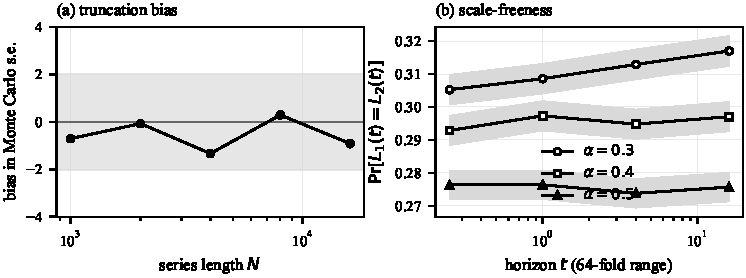
\includegraphics[width=5in]{fig_simulator}}
\vspace*{6pt}
\caption{Left: realized bias of the simulated normalized undershoot against its
exact Beta mean, in Monte Carlo standard errors, as a function of the series
length; the shaded band is $\pm2$. Right: the simultaneity atom over a
\simTratio{}-fold range of horizons, with two-standard-error bands, for three
values of $\alpha$.}
\label{fig:simulator}
\alttext{Left panel: bias fluctuating within two standard errors of zero as the
series length grows. Right panel: three nearly horizontal curves of atom
probability against horizon on a logarithmic axis.}
\end{figure}

\begin{remark}[a residual finite-$N$ effect]
At the smallest index studied, $\alpha=0.3$, the atom estimate drifts mildly
upward across horizons at $N=\simJumps$. Repeating the comparison at
$N=32{,}000$ removes it: the difference between the extreme horizons falls from
$+1.3$ to $-0.4$ standard errors. The drift is therefore a truncation effect,
not a failure of Proposition~\ref{prop:atom}, and it is why the self-similarity
$p$-values in Table~\ref{tab:selfsim} are weakest at small $\alpha$.
\end{remark}

\subsection*{Testing the evolution equation}

With independent Ornstein--Uhlenbeck factors and test function
$\varphi(y)=y_1y_2$, every term of \eqref{eq:local} reduces to the joint Laplace
transform $M(t)=\E[\exp(-\kappa_1H_1(t)-\kappa_2H_2(t))]$: the equation becomes
$M'(t) = -\E[(\kappa_1s_1+\kappa_2s_2)e^{-t(\kappa\cdot s)}]$ with
$s_j=H_j(t)/t$, and the tensorized alternative is \eqref{eq:tensor}. $M'(t)$ is
estimated by a central difference evaluated on the \emph{same} simulated paths
at $t\pm h$, which removes almost all Monte Carlo noise from the difference
quotient.

\subsection*{The correlation sweep}

The sweep of Table~\ref{tab:sweep} runs over
$\alpha_i,\alpha_h,\alpha_c\in\{0.2,0.35,0.5,0.65\}$,
$\sigma_i,\sigma_h\in\{0.5,1,2\}$, $a_i,a_h\in\{0.5,1,2\}$ and
$\kappa_i,\kappa_h,\kappa_0\in\{0.1,1,10\}$, on \sweepNdeltas{} horizons
geometrically spaced from \sweepDeltaLo{} to \sweepDeltaHi{}. The function
$\E[1-e^{-\kappa\Delta H}]$ is tabulated once by exact simulation on a
logarithmic grid of $\kappa$ and interpolated, so the sweep involves no further
simulation. A term structure is classified as rising if its maximum is at the
last horizon and its minimum at the first, falling in the mirror case, hump if
the maximum is interior, dip if the minimum is interior, and flat if the total
variation is below a relative tolerance of $10^{-4}$.

\subsection*{Duration estimators}

\emph{Hill.} For order statistics $\tau_{(1)}\ge\dots\ge\tau_{(n)}$ the Hill
estimator at threshold $k$ is
$\hat\alpha_k = (k^{-1}\sum_{i\le k}\log(\tau_{(i)}/\tau_{(k+1)}))^{-1}$
\citep{hil75}. We report the value at the flattest window of the Hill plot,
chosen as the run of nine consecutive $k$ minimizing the standard deviation of
$\hat\alpha_k$, which removes the arbitrary single-threshold choice. Zero
durations are retained: they count toward $n$ and hence toward the choice of
$k$, which is precisely the channel through which bursts bias the estimator.

\emph{Running mean.} The ratio of the sample mean over the second half of the
duration sequence to that over the first. For a finite mean this tends to one;
for an infinite mean it grows with sample size. It uses no threshold and no
parametric assumption.

\emph{Burst aggregation.} Given a window $W$, consecutive events whose
timestamps differ by less than $W$ are merged and durations recomputed. On HOSE
the analogous operation merges prints that share a one-second timestamp.

\emph{Diurnal adjustment.} Durations are divided by a smoothed profile of the
bin-wise mean duration over the observation window (48 bins for the
twenty-four-hour crypto sample, 24 for the HOSE session), interpolated across
empty bins, smoothed by a three-bin moving average and normalized to mean one.

\emph{Goodness of fit.} Following \citet{cla09}, $x_{\min}$ is chosen to
minimize the Kolmogorov--Smirnov distance, $\alpha$ is fitted by maximum
likelihood above it, and the $p$-value is obtained from parametric bootstrap
replications that resample the body non-parametrically and draw the tail from
the fitted power law. A small $p$-value rejects the power law; we treat
$p<0.10$ as rejection.

%%%%%%%%%%%%%%%%%%%%%%%%%%%%%%%%%%%%%%%%%%%%%%%%%%%%%%%%%%%%%%%%%%%%%%%%%%%%
\section{Reproduction}\label{app:repro}
%%%%%%%%%%%%%%%%%%%%%%%%%%%%%%%%%%%%%%%%%%%%%%%%%%%%%%%%%%%%%%%%%%%%%%%%%%%%

The accompanying repository contains the clock simulator and closed forms
(\texttt{src/nmf/}), the collectors for both data sets (\texttt{data/}), one
script per experiment (\texttt{experiments/}), and the code that converts the
resulting JSON into the tables, figures and numerical macros of this manuscript.
Every experiment is seeded, and every number quoted above is generated rather
than transcribed: rebuilding the paper from raw data requires running the
collectors, the experiment scripts, and \texttt{make}.

The crypto sample is one UTC day and the HOSE sample one morning session; both
are archived with the code, since public trade endpoints do not serve deep
history. The two limitations we regard as material are stated in the text: the
HOSE session is short, and its one-second timestamp resolution caps the finest
event definition available in that market.

\section*{Acknowledgments}

\section*{ORCID}

\noindent Quang-Vinh Dang -- \textcolor{red}{\textbf{[insert ORCID iD before
submission]}}

\begin{thebibliography}{99}

\bibitem[Ascione {\it et al.}(2024)]{asc24} G. Ascione, E. Scalas, B. Toaldo \&
L. Torricelli (2024) Time-changed Markov processes and coupled non-local
equations. arXiv:2412.14956.

\bibitem[Bacry {\it et al.}(2013)]{bac13} E. Bacry, S. Delattre, M. Hoffmann \&
J.-F. Muzy (2013) Modelling microstructure noise with mutually exciting point
processes, {\it Quantitative Finance} {\bf 13} (1), 65--77,
\url{https://doi.org/10.1080/14697688.2011.647054}.

\bibitem[Bandi {\it et al.}(2017)]{ban17} F. M. Bandi, D. Pirino \& R. Renò
(2017) EXcess idle time, {\it Econometrica} {\bf 85} (6), 1793--1846,
\url{https://doi.org/10.3982/ECTA13595}.

\bibitem[Barndorff-Nielsen {\it et al.}(2001)]{bar01} O. E. Barndorff-Nielsen,
J. Pedersen \& K. Sato (2001) Multivariate subordination, self-decomposability
and stability, {\it Advances in Applied Probability} {\bf 33} (1), 160--187,
\url{https://doi.org/10.1239/aap/999188322}.

\bibitem[Bertoin(1999)]{ber99} J. Bertoin (1999) Subordinators: examples and
applications. In: {\it Lectures on Probability Theory and Statistics
(Saint-Flour XXVII)}, Lecture Notes in Mathematics 1717, 1--91. Berlin:
Springer, \url{https://doi.org/10.1007/978-3-540-48115-7_1}.

\bibitem[Clark(1973)]{cla73} P. K. Clark (1973) A subordinated stochastic
process model with finite variance for speculative prices, {\it Econometrica}
{\bf 41} (1), 135--155, \url{https://doi.org/10.2307/1913889}.

\bibitem[Clauset {\it et al.}(2009)]{cla09} A. Clauset, C. R. Shalizi \&
M. E. J. Newman (2009) Power-law distributions in empirical data, {\it SIAM
Review} {\bf 51} (4), 661--703, \url{https://doi.org/10.1137/070710111}.

\bibitem[D'Onofrio {\it et al.}(2025)]{don25} G. D'Onofrio, G. Mutti \&
P. Semeraro (2025) Additive subordination of multiparameter Markov processes.
arXiv:2507.20863.

\bibitem[Dynkin(1961)]{dyn61} E. B. Dynkin (1961) Some limit theorems for sums
of independent random variables with infinite mathematical expectations. In:
{\it Selected Translations in Mathematical Statistics and Probability},
Volume 1, 171--189. Providence, Rhode Island: American Mathematical Society.

\bibitem[Engle \& Russell(1998)]{eng98} R. F. Engle \& J. R. Russell (1998)
Autoregressive conditional duration: a new model for irregularly spaced
transaction data, {\it Econometrica} {\bf 66} (5), 1127--1162,
\url{https://doi.org/10.2307/2999632}.

\bibitem[Gatheral {\it et al.}(2018)]{gat18} J. Gatheral, T. Jaisson \&
M. Rosenbaum (2018) Volatility is rough, {\it Quantitative Finance} {\bf 18}
(6), 933--949, \url{https://doi.org/10.1080/14697688.2017.1393551}.

\bibitem[Geman {\it et al.}(2001)]{gem01} H. Geman, D. B. Madan \& M. Yor
(2001) Time changes for Lévy processes, {\it Mathematical Finance} {\bf 11}
(1), 79--96, \url{https://doi.org/10.1111/1467-9965.00108}.

\bibitem[Hill(1975)]{hil75} B. M. Hill (1975) A simple general approach to
inference about the tail of a distribution, {\it The Annals of Statistics}
{\bf 3} (5), 1163--1174, \url{https://doi.org/10.1214/aos/1176343247}.

\bibitem[Lamperti(1958)]{lam58} J. Lamperti (1958) An occupation time theorem
for a class of stochastic processes, {\it Transactions of the American
Mathematical Society} {\bf 88} (2), 380--387,
\url{https://doi.org/10.2307/1993215}.

\bibitem[Lo \& MacKinlay(1990)]{lo90} A. W. Lo \& A. C. MacKinlay (1990) An
econometric analysis of nonsynchronous trading, {\it Journal of Econometrics}
{\bf 45} (1--2), 181--211,
\url{https://doi.org/10.1016/0304-4076(90)90098-E}.

\bibitem[Luciano \& Semeraro(2010)]{luc10} E. Luciano \& P. Semeraro (2010)
Multivariate time changes for Lévy asset models: characterization and
calibration, {\it Journal of Computational and Applied Mathematics} {\bf 233}
(8), 1937--1953, \url{https://doi.org/10.1016/j.cam.2009.09.028}.

\bibitem[Mainardi {\it et al.}(2000)]{mai00} F. Mainardi, M. Raberto,
R. Gorenflo \& E. Scalas (2000) Fractional calculus and continuous-time finance
II: the waiting-time distribution, {\it Physica A} {\bf 287} (3--4), 468--481,
\url{https://doi.org/10.1016/S0378-4371(00)00386-1}.

\bibitem[Marshall \& Olkin(1967)]{mar67} A. W. Marshall \& I. Olkin (1967) A
multivariate exponential distribution, {\it Journal of the American Statistical
Association} {\bf 62} (317), 30--44,
\url{https://doi.org/10.2307/2282907}.

\bibitem[Meerschaert \& Scheffler(2004)]{mee04} M. M. Meerschaert \&
H.-P. Scheffler (2004) Limit theorems for continuous-time random walks with
infinite mean waiting times, {\it Journal of Applied Probability} {\bf 41} (3),
623--638, \url{https://doi.org/10.1239/jap/1091543414}.

\bibitem[Meerschaert \& Sikorskii(2012)]{mee12} M. M. Meerschaert \&
A. Sikorskii (2012) {\it Stochastic Models for Fractional Calculus}. Berlin: De
Gruyter, \url{https://doi.org/10.1515/9783110258165}.

\bibitem[Olver {\it et al.}(2010)]{nist10} F. W. J. Olver, D. W. Lozier,
R. F. Boisvert \& C. W. Clark, eds. (2010) {\it NIST Handbook of Mathematical
Functions}. Cambridge: Cambridge University Press.

\bibitem[Rosiński(2007)]{ros07} J. Rosiński (2007) Tempering stable processes,
{\it Stochastic Processes and their Applications} {\bf 117} (6), 677--707,
\url{https://doi.org/10.1016/j.spa.2006.10.003}.

\bibitem[Scalas {\it et al.}(2000)]{sca00} E. Scalas, R. Gorenflo \&
F. Mainardi (2000) Fractional calculus and continuous-time finance, {\it
Physica A} {\bf 284} (1--4), 376--384,
\url{https://doi.org/10.1016/S0378-4371(00)00255-7}.

\bibitem[Semeraro(2008)]{sem08} P. Semeraro (2008) A multivariate variance
gamma model for financial applications, {\it International Journal of
Theoretical and Applied Finance} {\bf 11} (1), 1--18,
\url{https://doi.org/10.1142/S0219024908004701}.

\bibitem[Sun {\it et al.}(2017)]{sun17} Y. Sun, R. Mendoza-Arriaga \&
V. Linetsky (2017) Marshall--Olkin distributions, subordinators, efficient
simulation, and applications to credit risk, {\it Advances in Applied
Probability} {\bf 49} (2), 481--514,
\url{https://doi.org/10.1017/apr.2017.11}.

\bibitem[Toaldo(2015)]{toa15} B. Toaldo (2015) Convolution-type derivatives,
hitting-times of subordinators and time-changed $C_0$-semigroups, {\it
Potential Analysis} {\bf 42} (1), 115--140,
\url{https://doi.org/10.1007/s11118-014-9426-5}.

\end{thebibliography}

\end{document}
